%!TeX root = thesis-main.tex
% revisions
\newcommand{\LP}[2]{\marginpar{$\color{red}\star$}\color{gray}\sout{#1}\color{blue}\
  #2 \color{black}}
\newcommand{\LPr}[2]{{\color{gray}\ #1\ \color{orange}\  #2}}

%\lstset{frame=single,basewidth=0.5em,language={scafi},
%basicstyle=\lst@ifdisplaystyle\small\fi\ttfamily}

%\chapter{A Field-based Computing Approach to Sensing-driven Clustering in Robot Swarms}
\chapter[Sensing-driven Clustering in Swarms]{Sensing-driven Clustering in Swarms: A Field-based computing approach}\label{chap:eng:clustering}\mtcaddchapter
\minitoc% Creating an actual minitoc

\emph{Swarm intelligence}
 is the collective-level ability to solve problems
 in large groups of relatively simple agents that interact with each other locally, i.e., based on physical/logical proximity~\cite{DBLP:books/daglib/0032898}.
%
Common but not exhaustive classes of collective behaviours
 include spatial organization (e.g., pattern formation),
 swarm navigation,
 and collective-decision making~\cite{DBLP:journals/swarm/BrambillaFBD13}.
%

In particular, one problem of interest is \emph{swarm clustering} \cite{DBLP:conf/smc/LeeKK05,DBLP:journals/asc/CruzNM17},
 whereby the classical data clustering task
 (i.e., the unsupervised learning task where data items are grouped to promote intra-group similarity)
 is brought in swarm settings.
%
This problem revolves around splitting the swarm
 into groups of individuals, called \emph{clusters},
 such that the individuals in the same \emph{cluster}
 are more similar to each other (for some definition of \emph{similarity}) than to those in other clusters.
%
Once a cluster is formed, typically it is assigned a \emph{sub-goal} to be carried on collectively.
%
Typical clustering approaches may consider
 the spatial distribution of the individuals
 or the goals of the individuals to define clusters
 \rev{that represent, e.g.,} teams or interaction domains.
%
In this chapter, 
 we focus on \emph{sensing-based clustering}~\cite{DBLP:conf/ccnc/LinM07}, namely
 a clustering problem
 that considers both the spatial distribution of individuals
 and the environmental values sensed by these individuals (through sensors).
 This is essential for \ac{cpsw} applications due to the tight integration with the physical world.
%
That is, the goal is to seek clusters of neighbour individuals with a similar perception of some sensed value.
%
The problem can be in a \emph{static} form,
 where a snapshot of the system state is considered,
 or in a \emph{dynamic} form,
 where values change over time
 and solutions have to deal with change somehow.
%
The problem has been considered in Wireless Sensor Networks (WSNs) and Internet-of-Things (IoT) applications like
  environment monitoring and control~\cite{DBLP:conf/ccnc/LinM07},
  efficient distributed collection~\cite{DBLP:journals/ijcomsys/PhamLPC10},
  and disaster management~\cite{DBLP:journals/jaihc/KucukBSK20}.
%
However, to the best of our knowledge, 
 no existing work addresses the dynamic problem in \ac{cpsw}, which requires specific
techniques to adaptively re-adjust clusters to face changes.
%
Additionally, we look for solutions featuring \emph{resilience}, namely,
 leveraging distribution and decentralization to continuously face changes and faults, hence avoiding single points of failures and potential bottlenecks.
%
%Therefore, i
Accordingly, we present and address the \emph{dynamic sensing-based swarm clustering} problem,
 based on our language-based view of \ac{cpsw}, 
 namely enforcing the use of a field-based programming model, 
 both for the specification of the problem (i.e., the system model) and for the solution (i.e., the distributed aggregate computing program definition).  
%
%In this approach, computations
% leverage an execution model based on repeated computation
% and asynchronous neighbour-based communication.
%
%On top, complex collective behaviour is described in terms of
 %a  functional abstraction, namely, by
% functional manipulations of \emph{(computational) fields}, i.e.,
% data structures evolving over time that map agents in a domain to computational values---sort of % spatially distributed streams of values.
%
%This is inspired by the common notion of fields found in physics (e.g., force or magnetic fields).
%
%Notice, however, that in our viewpoint, the computational fields assign values to agents rather than to environment (space-time) positions as in e.g. \emph{artificial potential fields}~\cite{DBLP:conf/icra/Warren89},
% though the approaches are similar and related.
%
%It has shown to conveniently express
% a variety of \rev{resilient} collective swarm-like behaviour including
% self-healing distance estimation (\emph{gradient})~\cite{DBLP:conf/saso/AudritoCDV17},
% self-stabilising leader election~\cite{DBLP:conf/saso/MoBD18},
 %distributed collection~\cite{audrito2021jcee-distributed-collection},
% and team creation and coordination~\cite{DBLP:journals/eaai/CasadeiVAPD21}---and to scale with complexity up to high-level composite patterns~\cite{DBLP:journals/fgcs/PianiniCVN21}.

Essentially, the core idea of our clustering approach is to make agents
 in local \rev{minima (or maxima)} of the sensed value \rev{(depending on whether lowest or highest values are most significant)} spawn a spatial process of gathering for neighbour devices until finding the proper size of the cluster,
 additionally managing interactions with other clusters when there are overlaps.
%

%\section{Background and Motivation}
\label{s:background}
%\meta{cross-disciplinary approaches $\to$ fields?}

\section{Field-based Concurrent Processes}
\sloppy
Field-based concurrent processes, also called \emph{aggregate processes}~\cite{DBLP:conf/coordination/CasadeiVAPD19,DBLP:journals/eaai/CasadeiVAPD21},
 are field-based computations
 that exist dynamically:
 they can be dynamically generated (usually by individual agents),
 execute on a dynamic set of agents,
 and disappear once all its members withdraw.
%
They have been formalized in \cite{DBLP:conf/coordination/CasadeiVAPD19}
 and deeply covered in \cite{DBLP:journals/eaai/CasadeiVAPD21},
 showing how they can support the design of intelligent collective behaviour by extending the practical expressiveness of field-based programming models~\cite{DBLP:journals/jlap/ViroliBDACP19}.
%
We provide a brief account of the details relevant for this chapter in the following.

Indeed, the aggregate process abstraction
 is relevant since an aggregate process instance,
 by running on a (evolving) subset of the agents,
 can be used to denote a \emph{dynamic} cluster.
%
Therefore, clustering algorithms
 can be expressed in terms of how
 aggregate processes are generated (candidate cluster formation)
 and
 merged/removed (cluster selection).

Aggregate processes can be expressed as normal field-based functions and spawned through a \lstinline|spawn| construct
 with the following signature:
%
\begin{lstlisting}
// spawn is a generic function which accepts 3 parameters
def spawn[K,A,R](process: K => A => (R,Boolean),
                 newProcesses: Set[K],
                 args: A): Map[K,R]
\end{lstlisting}
%
The generic type \lstinline|K| instantiates to the type of \emph{process key}, 
 also called a \emph{process identifier (PID)}, which also works as construction parameter;
 the generic type \lstinline|A| instantiates to the type of runtime parameters for the currently running process instances;
 the generic type \lstinline|R| instantiates to the type of the output of the process.
%
A \emph{process definition} has curried type \lstinline|K => A => (R,Boolean)|, 
namely a function from a value of type \lstinline|K| and a value of type \lstinline|A| to a pair of a value of type \lstinline|R| and a Boolean.
%
The Boolean value, called the \emph{process status}, 
 expresses if the device that has executed a given process instance
 would like to participate in the process (\lstinline|true| status)
 or not (\lstinline|false| status).
%
The crucial point is that every device that participates in a process with PID $\pi$ automatically propagates the process PID $\pi$ to all its neighbours, 
which will run a corresponding process instance when the \lstinline|spawn| function is evaluated.
%
So, the \lstinline|spawn| function accepts a function \lstinline|process| of a field-based behaviour,
 a set \lstinline|newProcesses| of new process instances to be generated locally in the current round,
 and a value of type \lstinline|A| for the runtime input of the instances currently running in the local round of a given device.
%
Notice that, though \lstinline|process| can be a field of functions, 
 it is typically a constant field of the same function, 
 which means that usually a \lstinline|spawn| expression enables running zero or more process instances of the same kind of process.
%
Evaluation of \lstinline|spawn| returns a \lstinline|Map[K,R]|
 (i.e., a hashmap or dictionary) which is a set of entries
 mapping the PIDs of executed process instances (with status \lstinline|true|) to corresponding outputs of type \lstinline|R|.
%

As an example, consider building a separate gradient computation
 for each distinct source agent, that will expand within a certain range $\rho$. 
 This could be coded as follows in ScaFi:
\begin{lstlisting}[mathescape]
type DeviceId = Int
// Process definition as a function
val proc: DeviceId => Boolean => (Double, Boolean) = id => isSource => {
  val output = gradient(id == deviceId())
  val status = if(id == deviceId()) isSource
               else output < $\rho$
  (output, status)
}
// Set of processes to be generated locally
val newProcesses: Set[DeviceId] =
  if(isSource()) Set(deviceId()) else Set.empty
// Expression for handling acquired and generated processes
val gradients: Map[DeviceId,Double] =
  spawn[DeviceId,Boolean,Double](process, newProcesses, isSource())
\end{lstlisting}
%
\rev{In detail, the IDs of sources are used as PIDs; so, for instance, a gradient from agent 7 will become a process with PID 7. The process logic is defined through \lstinline|proc|, which is a function of the PID \lstinline|id| and Boolean argument \lstinline|isSource| denoting whether the running agent is a source, as provided by built-in sensor function \lstinline|isSource()|. In \lstinline|proc|, a gradient is built from the agent whose ID, provided by \lstinline|deviceId()|, matches the \lstinline|id| of the source corresponding to the current process instance. Then, \lstinline|status| is defined \lstinline|true| if the source for the process is still a source or, for non-source agents, if their gradient value is lower than threshold $\rho$. Notice that when the original source is not a source any more, the gradient \lstinline|output| will rise, eventually causing all the agents to leave that process.
%
Value \lstinline|newProcesses| will be a singleton set 
 with the ID of the running device
 when its \lstinline|isSource()| sensor returns true,
 or the empty set otherwise.
%
In the former case, 
 a corresponding process is spawned
 if it did not already exist.
%
The evaluation of the \lstinline|spawn| call, then,
 will run both new and existing processes
 including those executed (and not quit) at the previous round,
  as well as those acquired from neighbours.
%
The output of the \lstinline|spawn| expression
 will be a map from the PIDs of the processes locally executed
 to the value of the gradient (\lstinline|output|) locally computed in those process instances.
}

An example of the dynamics of such a program is provided in \Cref{fig:spawn-dynamics}.
%
In the picture: nodes are agents; labels on nodes are agent IDs; edges denote neighbouring links, over which messages are sent and received; the output of the \lstinline|spawn| expression is shown above the nodes unless it is an empty map (not shown); the different sub-pictures are snapshots of a corresponding hypothetical system state trajectory that may result after multiple rounds of execution in multiple devices.
%
A more thorough introduction and description of aggregate processes together with more examples is available in \cite{DBLP:journals/eaai/CasadeiVAPD21}.

\begin{figure}
\centering
\subfloat[Initial network.\label{fig:spawn-dynamics-a}]{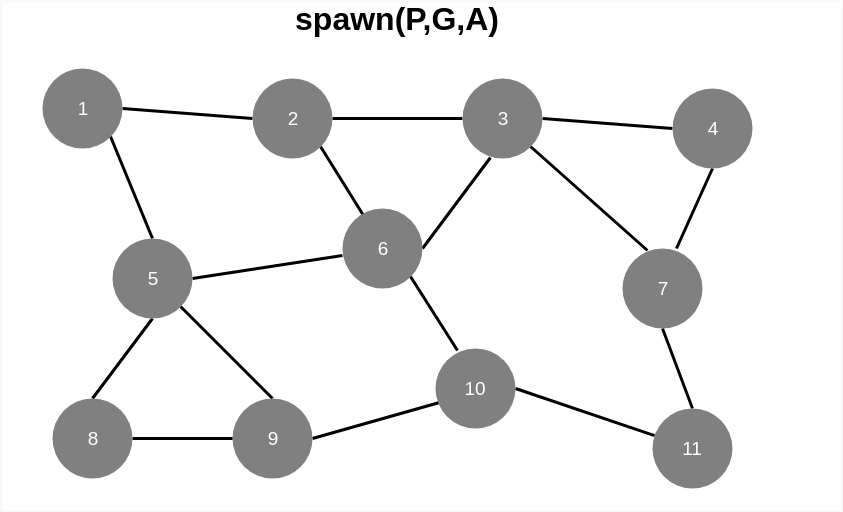
\includegraphics[width=0.45\textwidth]{papers/swarm-intelligence2021/img/spawn-dynamics1.png}}\hfill
%
\subfloat[A process is generated on agent $1$.\label{fig:spawn-dynamics-b}]{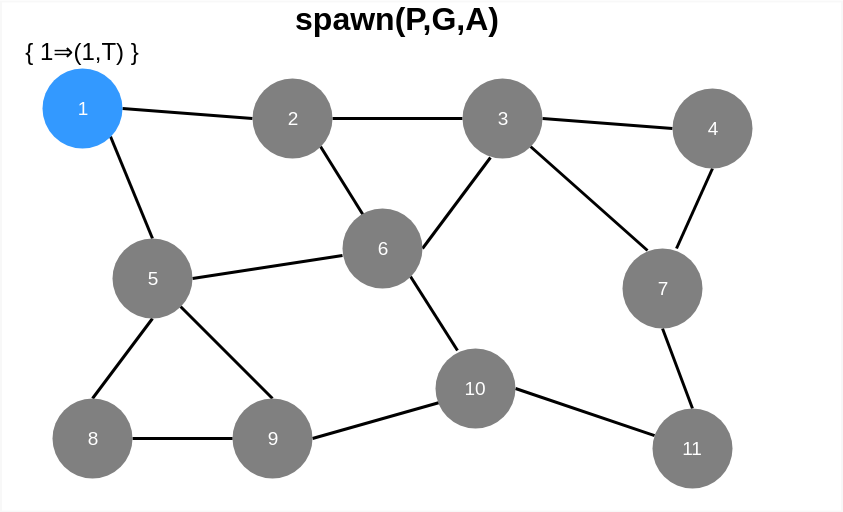
\includegraphics[width=0.45\textwidth]{papers/swarm-intelligence2021/img/spawn-dynamics2.png}}\\
%
\subfloat[The process with PID $1$ propagates up to a certain range.\label{fig:spawn-dynamics-c}]{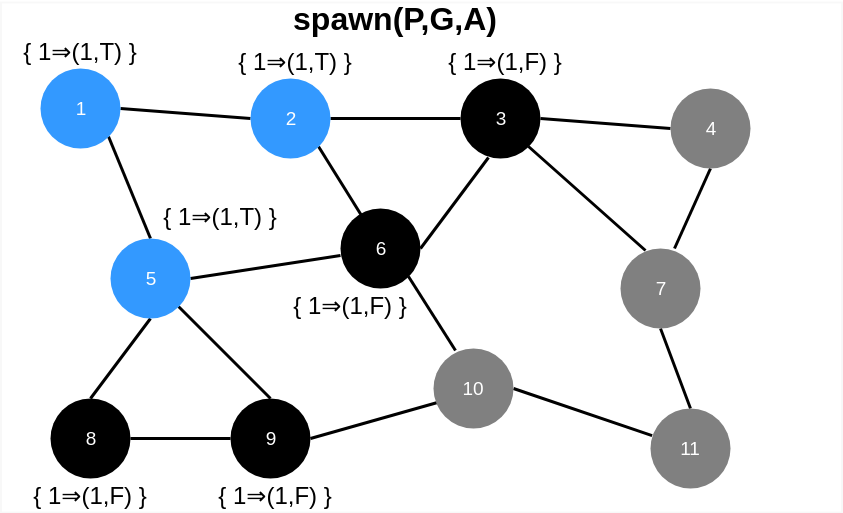
\includegraphics[width=0.45\textwidth]{papers/swarm-intelligence2021/img/spawn-dynamics3.png}}\hfill
%
\subfloat[The ``border'' of a process can change dynamically.\label{fig:spawn-dynamics-d}]{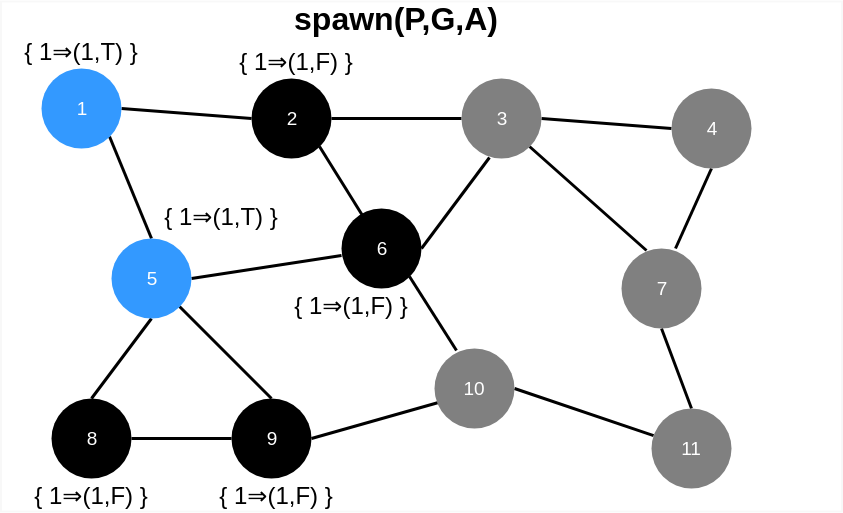
\includegraphics[width=0.45\textwidth]{papers/swarm-intelligence2021/img/spawn-dynamics4.png}}\\
%
\subfloat[Another process is spawned by source agent $3$.\label{fig:spawn-dynamics-e}]{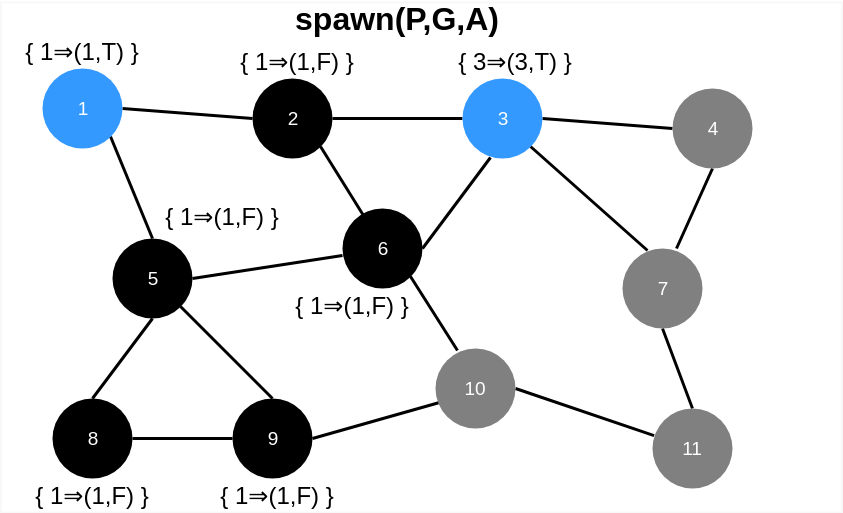
\includegraphics[width=0.45\textwidth]{papers/swarm-intelligence2021/img/spawn-dynamics5.png}}\hfill
%
\subfloat[Processes can overlap. Agents $2$ and $6$ run the two processes with PID $1$ and $3$.\label{fig:spawn-dynamics-f}]{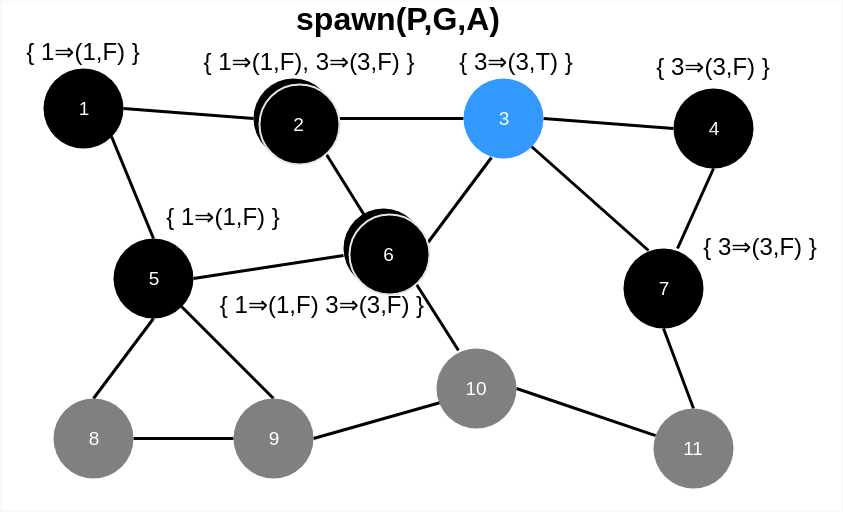
\includegraphics[width=0.45\textwidth]{papers/swarm-intelligence2021/img/spawn-dynamics6.png}}\\
%
\subfloat[Process $1$ ceases to exist.\label{fig:spawn-dynamics-g}]{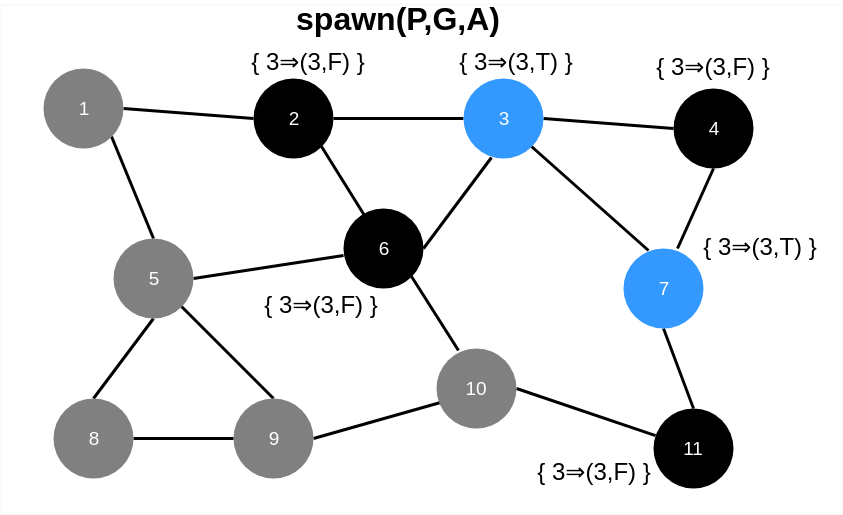
\includegraphics[width=0.45\textwidth]{papers/swarm-intelligence2021/img/spawn-dynamics7.png}}
%
\caption{Examples of the dynamics of multiple concurrent gradient processes.}
\label{fig:spawn-dynamics}
\end{figure}


\section{Resilient Dynamic Cluster Formation}
\label{s:background-clustering}

Different cluster models exist
 and, for each cluster model, several algorithms can be devised~\cite{DBLP:journals/sigkdd/Estivill-Castro02}.
%
These are reviewed and compared with our cluster model in \Cref{s:rw}.

In this chapter, we focus on \emph{swarm clustering},
 which involves associating each swarm member
 to zero or more clusters.
%
So, this is a problem of \emph{cluster formation}~\cite{DBLP:journals/tie/GeHZ18},
 more than a problem of \emph{cluster analysis} (which generally includes cluster formation followed by cluster evaluation).
%
A \emph{cluster}, in this setting,
 is essentially a label (\emph{cluster ID}),
 which can be associated to an agent,
 and that can be used to determine its behaviour.
%
In field terms,
 a clustering can be seen as a field
 mapping each agent to
 a set of cluster IDs---we call this a \emph{clustering field}.

Essentially, a cluster can be used to determine, query, and control a group of agents.
%
Such a group could represent a team, used for cooperation or to solve a common goal,
 or a space-time domain for a field computation.
%
Indeed, as the agents are situated in space,
 they provide a means for extracting data
 from their corresponding location,
 which may be instrumental for environment monitoring,
 data acquisition, etc.

Moreover, we consider \emph{dynamic clustering}~\cite{DBLP:journals/pr/RoaTG19},
 where the emphasis is not on identifying a single clustering
 for a given system configuration,
 but to update and evolve a clustering solution
 as the system configuration evolves
 (e.g., due to mobility, failure, or change in other clustering criteria).
%
The specific problem we tackle is \emph{dynamic sensing-based/space-based swarm clustering},
 which involves associating each swarm member
 to zero or more clusters, and to evolve such association by considering change in the environment (\emph{sensing-based}) and spatial location of the members (\emph{space-based}).
%

In summary, our goal is to define a distributed, decentralized, field-based
 clustering algorithm,
 for the system model based on our language-based view
 described in \Cref{ssec:background:sysmodel},
 able to create and dynamically maintain a clustering field\rev{, resiliently}.
%
\rev{
Our focus on resilience 
 make centralized approaches not appropriate 
 since we cannot assume that some nodes 
 are infallible or always available.
}
%
%This model is different from other clustering models and algorithms as follows.
%%
%\begin{itemize}
%\item Our model differs from \emph{connectivity-based clustering}
% as the topology is already given (neighbourhood-based).
%\end{itemize}
%
This work draws motivation
 from
 (i) the relevance of the problem for \emph{situated} systems as \ac{cpsw},
 (ii) a scarcity of solutions to the problem of \emph{sensing-driven spatial clustering} in literature,
 and
 (iii) a general lack of effective field-based clustering solutions.
%
Refer to \Cref{s:rw} for a more detailed account on these research gaps.


\section{Sensing-Driven Clustering}
\label{s:contrib}

%\meta{ASSIGNED TO: Giorgio (interacting with G. Aguzzi/Ferruccio)}

\rev{
In this section,
 after describing a minimal set of \emph{assumptions}
 underlying the approach (\Cref{ssec:assumptions}),
 we define the \emph{problem} to be addressed (\Cref{ssec:problem-def}), in terms of inputs, outputs, and parameters,
 describe a specific instantiation of the problem for \emph{centroid-based} clustering on numeric values (\Cref{ssec:instantiation}),
 and then present a meta-algorithm providing a solution to the stated problem (\Cref{ssec:meta-algo}).
}


\rev{
\subsection{Assumptions}
\label{ssec:assumptions}
Before formally defining the problem of {\em Dynamic Sensing Based Swarm Clustering}, we summarize the assumptions about the swarm devices and the environment in which they act. Such assumptions justify both the way we define the problem, and some of the design choices we adopt for its solution.
%
\begin{enumerate}
\item A {\em swarm} is composed by a set of possibly many relatively simple autonomous cyber-physical agents, %(e.g., ground, airborne, underwater).
\item An {\em agent} can move within the environment, sense, and actuate.
\item {\em Communication} is based on  peer-to-peer connection link, based on the proximity of agents, without relying on infrastructure (e.g., LTE network, Wi-Fi network).
\item {\em Reliability} of agents themselves and communications are not guaranteed and, in some scenarios, failures are  quite likely.
\item The measures of the {\em environment}, as sensed by the agents, can change over time.
\item The measures of interest of the {\em environment} at two points in space close to each other tend to be positively correlated.
\end{enumerate}
%
The above assumptions, based on our system model defined in \Cref{part:background}, 
 are rather weak and, therefore, quite challenging. 
 They encompass scenarios where a swarm of agents explores an area where multiple natural phenomena are happening. Therefore, even if the proposed solution target \ac{cpsw}, it can be applied to other scenarios, such as WSNs and IoT, where the above assumptions are satisfied.

The field-based clustering algorithm for solving the {\em Dynamic Sensing Based Swarm Clustering} problem will be discussed below. For now, we just want to point out that our assumptions justify a fully distributed approach in which agents exchange information with their neighbours.

First, given the very nature of swarm systems, 
 problems are usually better solved by distributed algorithms than centralized algorithms, e.g., \cite{hoshino:2013,DBLP:journals/asc/CruzNM17}. 
 In particular, by our assumption that agents and communications can fail, 
 and that there is no global communication infrastructure, 
 a node in charge of all the computations (either an agent or a base station) 
 would constitute a risky single point of failure. 
 Even if the swarm was able to recover from such failure by automatically choosing another central node, the switch would be cumbersome and potentially very costly, only to reach again a situation with another single point of failure.

Given agents whose connection links are established and lost based on the proximity with other agents, 
 it may be possible to build an abstraction on top of that, 
 whereby multi-hop communications are transparent, 
 and each agent has the illusion of being able to immediately communicate with any other agent in the swarm by specifying an appropriate ID 
 (this is, e.g., the typical abstraction brought by the IP layer of the TCP/IP stack). 
 While the cost of adding such an additional layer may be acceptable in some situations, for the specific goal of clustering this would not bring any advantage: as we shall see in the sections below, clusters spring out, expand, and collapse following spatial vicinity---i.e., a new cluster expands first to the immediate neighbours of the agent that generated it, and then progressively incrementally spreads to further agents.
}

\subsection{Problem Definition}\label{ssec:problem-def}

We address the problem of situation awareness and recognition, where a value distributed in space (e.g., temperature as measured by sensors) has to be monitored,
 by recognizing compact clusters with similar values (e.g., spatial regions with a similar temperature).
 This problem, called \emph{sensing-driven clustering} in literature, has been investigated largely in static scenarios \cite{DBLP:journals/jaihc/KucukBSK20,DBLP:journals/ijcomsys/PhamLPC10,DBLP:conf/ccnc/LinM07},
 where data from a fixed sensor network has to be processed to obtain the relevant clusters.
 However, solutions for such networks do not extend well to dynamic contexts, such as a mobile \acp{cpsw} system monitoring an environment:
 in this scenario, mobility and proximity of communication are key,
 and need to be handled by an algorithm that is resilient to changes in values, network structure and placement in space.
 To the best of our knowledge, this problem has never been previously considered in the literature.

A sensing-driven clustering algorithm for such system could be useful for several outcomes.
 Clusters may provide a compressed summary of the value distribution in space,
 to upload on the cloud and be graphically represented for human convenience.
%
Clusters may also be used to drive more complex situation recognition patterns:
 algorithms to detect dangerous situations may be run in each cluster separately,
 using information from that cluster to reach a verdict, 
 without interference from information on neighbouring clusters.
 Clusters may also be used to drive task assignments to the monitoring drones,
 possibly guiding their placement in space, by directing more drones in clusters where the need arises.

More formally, we consider the following problem:
\begin{itemize}
	\item \textbf{Input:} for each device, a unique identifier $i$ and a \emph{value} $v_i$ of type $T$ \rev{(possibly obtained through a sensor reading);}
	\item \textbf{Output:} for each device, a list of clusters to which the device belongs, represented as a map from unique identifiers $l$ of cluster leaders to corresponding cluster summary values $w^l$ of type $S$.
\end{itemize}
To formally specify the output, 
 we need some further details characterizing what a \emph{cluster} is, 
 how they should be selected, and what is their \emph{summary}. 
 This is attained through the following problem parameters.
\begin{itemize}
	\item \textbf{Metric:} a data type $M$ with
	\begin{itemize}
		\item a \emph{null} value $0_M$;
		\item a partial order\footnote{A partial order is a reflexive, transitive and anti-symmetric relation; with no requirement that either $x \leq y$ or $y \leq x$ for $x,y$ of type $M$.} $x \leq y$ defined for $x,y$ of type $M$;
		\item an addition operator $x + y$ defined for $x,y$ of type $M$, such that $x + 0_M = x$ and $x + y > x$ if $y > 0_M$;
		\item a positive function $d(i, j) > 0_M$ returning a value in $M$ representing a distance between a device $i$ and $j$ (depending on the devices' sensor states and possibly values $v_i$). \rev{This is intended to make use of spatial distance estimates as well as other factors (i.e., value distances).}
	\end{itemize}
	\item \textbf{Summary:} a data type $S$ with
	\begin{itemize}
		\item a value $s(i)$ of type $S$ in every device $i$ (depending on sensor state);
		\item an associative and commutative function $f : (S,S) \to S$, used to aggregate values $s(i)$ for devices in a same cluster.
	\end{itemize}
	\item \textbf{Leader selection:}
	\begin{itemize}
		\item a candidate radius $r(i)$ in $M$ (depending on sensor state and values), so that only devices with a relative distance strictly lower than $r(i)$ can belong to a cluster whose leader is $i$;\footnote{Notice that $r(i) = 0_M$ implies that no device can be in a cluster whose leader is $i$.}
		\item a commutative similarity predicate $p : (S,S) \to \{\top, \bot\}$, identifying similar clusters based on their summary.
	\end{itemize}
\end{itemize}
According to this description, a candidate cluster $\mathcal{C}$ is a set of devices with a leader $i$,
 such that every $j \in \mathcal{C}$ is within a distance of $r(i)$ from the leader $i$,
 according to the metric given by $d$.
 The summary $w_i$ of such cluster is the repeated aggregation through $f$ of the values $\{v_j : ~ j \in \mathcal{C}\}$.
 Nearby clusters are merged if their summaries are similar according to predicate $p$,
 and in such cases, the lowest identifier is selected as the leader of the merged cluster.

\rev{
Leaders are used to regulating clusters via aggregate processes and to easily support consistent coordination and decision-making regarding the activity of a cluster.
%
Notice that agents 
 may belong to multiple clusters:
 this is important to support 
 tracking phenomena that are spatially close to each other.
%
Indeed, if a node is in between two phenomena,
 it could participate in the corresponding clusters 
 at the same time to help to track
 or handle both phenomena.
}
%
We highlight that we aim to solve this problem by an \emph{adaptive} algorithm,
 that is, a program that is able to handle changes in its input, by periodically and asynchronously updating its internal values.

\subsection{Adaptive Centroid-based Clustering on Numeric Values} \label{ssec:instantiation}

In the evaluation section, we consider a specific instantiation of the \rev{parameters just introduced,}
 for centroid-based clustering on numeric values.
 In this context, the metric is a simple distance on values, so that $d(i, j) = \lvert v_i - v_j \rvert$.
 To prevent the creation of a candidate cluster for every device, 
 the candidate radius $r(i)$ is set to zero whenever $i$ is not a local minimum
 (i.e., has a neighbouring device $j$ such that $v_j < v_i$). 
 If instead $i$ is a local minimum, $r(i)$ is set to a fixed difference value $\theta$.
 The values $s(i)$ to be summarized are set to a tuple $[x_i, y_i, v_i, 1]$ of the devices' positions\footnote{We assume that a GPS-like sensor is available.} and values with the number 1,
 with an aggregator function $f$ that is a component-wise sum, so that the overall aggregate of a cluster $\mathcal{C}$ is (eventually) equal to the tuple
 $[\sum_{i \in \mathcal{C}} x_i, \sum_{i \in \mathcal{C}} y_i, \sum_{i \in \mathcal{C}} v_i, \#\mathcal{C}]$ (where $\#\mathcal{C}$ is the actual number of members of cluster $C$).
 The similarity predicate $p$ then declares two clusters as similar if they have centroids within a radius of $\gamma$,
 in a 3D space mixing spatial coordinates with a value coordinate:
\[
p([x, y, v, n], [x', y', v', n']) \quad\coloneqq\quad \lVert \frac{(x,y,v)}{n} - \frac{(x',y',v')}{n'} \rVert < \gamma
\]
where $(x,y,v)$ denotes a 3D vector and $\lVert \cdot \rVert$ denotes the norm of a vector.
 By setting the problem parameters as described, the meta-algorithm can select clusters of similar value,
 led by their minima, and merge overlapping clusters that are too close together and with a similar value.

\subsection{Adaptive Clustering Meta-Algorithm}
\label{ssec:meta-algo}

We now describe \rev{the general} meta-algorithm for the stated problem through state equations.
 The algorithm state is distributed, hence composed of variables $x_i$ depending on a device identifier $i$:
 we assume that such a variable is stored in device $i$ and periodically updated by it through the state equations.
%
Each equation may involve inspecting the state of variables in neighbour devices $j$:
 we assume that every device periodically shares its state with neighbours,
 so that a (not necessarily updated) view of neighbours' state is available in each device,
 and each state equation can be computed locally in the current device $i$, without remote memory accesses.
%
We use $\mathcal{N}(i)$ to denote the set of current neighbours of device $i$, i.e., the set of devices $j$ for which a view of their state is locally available in $i$ (not including $i$ itself).
 The execution of state equations can be performed in asynchronous rounds, as described in \Cref{part:background}.
 %
 \rev{In order to showcase the algorithm at work by examples, in the following we consider a network of three interconnected devices $i=0,1,2$, so that $\mathcal{N}(0) = \mathcal{N}(1) = \mathcal{N}(2) = \{0,1,2\}$. 
  We assume that the devices are placed in positions $(x_0, y_0) = (0,0)$, $(x_1, y_1) = (1,1)$, $(x_2,y_2) = (2,0)$ and hold values $v_0 = 2$, $v_1 = 3$, $v_2 = 1$. 
  We will also assume that the parameters are as described in Section \ref{ssec:instantiation}, with $\theta = \gamma = 3$.}

\begin{table}
\begin{tabular}{clcl}
$i$ & current device &
$\mathcal{N}(i)$ & neighbour set \\
$\ell$ & candidate leader &
$\mathcal{S}_i$ & candidate leader set \\
$m^\ell_i$ & metric in $i$ from $\ell$ &
$c^\ell_i$ & whether $i$ belongs to cluster $\ell$ \\
$p^\ell_i$ & parent of $i$ in cluster $\ell$ &
$t^\ell_i$ & partial summary in $i$ for cluster $\ell$ \\
$u^\ell_i$ & candidate leader summary in $i$ for $\ell$ \\
$l_i$ & selected leader for cluster $i$, if any &
$w_i$ & selected summary for cluster $i$, if any \\
$l^\ell_i$ & selected leader for cluster $\ell$ in $i$ &
$w^\ell_i$ & selected summary for cluster $\ell$ in $i$
\end{tabular}
\caption{State variables used in the state equations.} \label{tab:variables}
\end{table}

\Cref{tab:variables} summarizes the state variables used in state equations.
 Every device maintains a candidate leader set $\mathcal{S}_i$, of possible clusters to which the device may belong. Every round, this set is updated as:
\[
\mathcal{S}_i ~=~ \{ \ell \in \mathcal{S}_j \text{ for } j \in \mathcal{N}(i) \text{ s.t. } c^\ell_j = \top \} \cup \begin{cases}
	\emptyset & \text{if } r(i) = 0_M \\
	\{ i \} & \text{otherwise}
\end{cases}
\]
Thus, $\mathcal{S}_i$ includes $i$ provided that $r(i) > 0_M$, together with other candidate leaders $\ell$ considered by neighbours
 (in their candidate leader set and which have computed to be within the cluster).
 In field-based computing, this set is implicitly maintained by the \emph{spawn} construct,
 given $c^\ell_i$ as process return status and $\{ i \}$ as new process key (if $r(i) > 0_M$).
 %
\rev{In our sample network, the initial value for $\mathcal{S}_i$ in each $i$ will only consider the current device, as information from neighbouring devices is not available yet. Thus, we will have $\mathcal{S}_0 = \{0\}, \mathcal{S}_1 = \{\}, \mathcal{S}_2 = \{2\}$. After convergence, each node will understand itself as possibly belonging to clusters 0 and 2, so that $\mathcal{S}_0 = \mathcal{S}_1 = \mathcal{S}_2 = \{0,2\}$.}

Most of the meta-algorithm computation is repeated for each of the candidate leaders $\ell \in \mathcal{S}_i$. First, a metric $m^\ell_i$ of the distance between $\ell$ and $i$ is computed,
 through the following equation (i.e., the \lstinline|gradient| block in field-based computing---cf. \Cref{sec:field-calculus-building-blocks}):
\[
m^\ell_i = \begin{cases}
	0_M & \text{if } \ell = i \\
	\min \{m^\ell_j + d(i,j) : ~ j \in \mathcal{N}(i) \} & \text{otherwise}
\end{cases}
\]
\rev{In the sample network, we will have $m^0_0 = m^2_2 = 0$, $m^0_1 = 0 + \vert v_0 - v_1 \vert = 1$, $m^2_1 = 0 + \vert v_2 - v_1 \vert = 2$, $m^2_0 = m^0_2 = 0 + \vert v_0 - v_1 \vert + \vert v_2 - v_1 \vert = 3$. From $m^\ell_i$, we also decide the values $c^\ell_i$ as the truth predicates of whether $m^\ell_i \leq \theta$.}

Then, an optional parent $p^\ell_i$ for $\ell \neq i$ is determined as the neighbour $j$ with minimal $m^\ell_j$ (resolving ties by the identifier $j$ itself):
\[
p^\ell_i = \begin{cases}
	\arg\min_{j \in \mathcal{N}(i)} \{ (m^\ell_j, j) \} & \text{if } \ell \neq i \\
	\text{None} & \text{otherwise}
\end{cases}
\]
\rev{In our example, we have that $p^0_1 = 0$, $p^2_1 = 2$, $p^2_0 = p^0_2 = 1$ while $p^0_0$ and $p^2_2$ are undefined.}
Through it, partial summaries $t^\ell_i$ can be computed (\lstinline|C| block in field-based computing---cf. \Cref{sec:field-calculus-building-blocks}):
\[
t^\ell_i = \text{reduce}(\{s(i)\} \cup \{t^\ell_j :~ j \in \mathcal{N}(i) \text{ and } p^\ell_j = i\}, f)
\]
where ``reduce'' is a function accumulating every element of a given set with the given binary function,
 and thus aggregates with $f$ the value $s(i)$ together with the $t^\ell_j$ values of neighbours $j$ which chose the current device $i$ as their parent.
%
\rev{In the sample network, we will have that $t^2_0 = s(0) = (0,0,2,1)$, $t^0_2 = s(2) = (2,0,1,1)$, $t^0_1 = s(1)+s(2)$, $t^2_1 = s(1)+s(0)$, $t^0_0 = t^2_2 = s(0)+s(1)+s(2) = (3,1,6,3)$.}
%
The value of the partial summary in the leader is then propagated through the cluster by a broadcast function:
\[
u^\ell_i = \begin{cases}
	t^\ell_i & \text{if } \ell = i \\
	u^\ell_{p^\ell_i} & \text{otherwise}
\end{cases}
\]
\rev{so that, in our example after convergence, each $u^\ell_i$ is $(3,1,6,3)$.}
Every candidate leader $i$ with $r(i) > 0_M$ is now able to choose its selected leader $l_i$,
 as the minimum candidate leader $j$ (possibly $i$ itself) with a summary similar to that of $i$ according to predicate $p$:
\[
(l_i, w_i) = \begin{cases}
	\min \{(\ell, u^\ell_i) :~ \ell \in \mathcal{S}_i \text{ and } p(u^\ell_i, u^i_i)\} & \text{if } r(i) > 0_M \\
	\text{None} & \text{otherwise}
\end{cases}
\]
\rev{In the running example, we will have that $l_0 = l_2 = 0$, $w_0 = w_2 = (3,1,6,3)$, since the two clusters are fully overlapping hence $p$ is true.}
The selected leader $l_i$ and corresponding summary $w_i$ is then propagated by broadcast through the cluster of $i$. For every $\ell \in \mathcal{S}_i$:
\[
(l^\ell_i, w^\ell_i) = \begin{cases}
	(l_i, w_i) & \text{if } \ell = i \\
	(l^\ell_{p^\ell_i}, w^\ell_{p^\ell_i}) & \text{otherwise}
\end{cases}
\]
Finally, in every device $i$, the meta-algorithm output is the map:
\[
\{ l^\ell_i \mapsto w^\ell_i :~ \ell \in \mathcal{S}_i \}.
\]

\begin{figure}
\begin{lstlisting}[escapechar=\%, caption=\scafi{} pseudo-code of the clustering meta-algorithm, label={fig:pseudocode}]
// process starts when %$r(i)$% is positive
val newProc = mux (%$r(i)$% > 0) { Set(mid) } { Set.empty }
// collect map from %$\ell \in $% to %$(m^\ell_i, u^\ell_i)$%
val clusters = spawn(%$\ell$% => _ => {
  val %$m^\ell_i$% = gradient(mid == %$\ell$%, %$d$%) // distance estimation
  val %$c^\ell_i$% = %$m^\ell_i$% < %$r(\ell)$% // whether device is in cluster
  val %$t^\ell_i$% = C(%$m^\ell_i$%, %$f$%, %$s(i)$%) // summary collection
  val %$u^\ell_i$% = broadcast(%$m^\ell_i$%, %$t^\ell_i$%) // summary broadcast
  return ((%$m^\ell_i$%, %$u^\ell_i$%), %$c^\ell_i$%) // process result and status
}, newProc, ())
// selected leader
val %$l_i$% = mux (%$r(i)$% > 0) {
  clusters.filter(x => %$p$%(x._2, clusters(mid))).keys.min
} { mid }
// selected leader summary
val %$w_i$% = mux (%$r(i)$% > 0) { clusters(%$l_i$%)._2 } { None }
// propagate in process
val result = spawn(%$\ell$% => _ => {
  val %$m^\ell_i$% = clusters(%$\ell$%)._1 // recover distances
  val %$c^\ell_i$% = %$m^\ell_i$% < %$r(\ell)$% // whether device is in cluster
  val (%$l^\ell_i$%, %$w^\ell_i$%) = broadcast(%$m^\ell_i$%, (%$l_i$%, %$w_i$%)) // final broadcast
  return ((%$l^\ell_i$%, %$w^\ell_i$%), %$c^\ell_i$%) // process result and status
}, newProc, ())
// build result map
return result.map(x => { x._2._1 -> x._2._2 })
\end{lstlisting}
\end{figure}

This meta-algorithm is presented as \scafi{} pseudo-code in \Cref{fig:pseudocode}, using \scafi{} library functions \lstinline|gradient|, \lstinline|C|, and \lstinline|broadcast|---cf. \Cref{sec:field-calculus-building-blocks}.
%
\rev{Notice that since clusters are represented as aggregate processes, and aggregate processes define ``scopes'' for collective computations, the participation of an agent in an aggregate process has by itself the information about the cluster membership; so, collective tasks may be assigned to any cluster, and these will be inherently played by all the members of that cluster.
}
%
 We also remark that although values $v_i$ are not directly used by the meta-algorithms, the parameters $r(i)$ and $d(i,j)$ are allowed to depend on them (and usually do),
 so that values are indirectly used. An example of such behaviour is given in the next section.

%figura della composizione blocchi?
%vedi anche: https://github.com/metaphori/paper-2021-swarm-intelligence-si/blob/master/_Brainstorming/algorithm2.md

\section{Evaluation}
\label{s:eval}

%\meta{ASSIGNED TO: G. Aguzzi / Roby}

In this section, we evaluate the meta-algorithm proposed in \Cref{ssec:meta-algo}
 in a case study of situation recognition within a synthetic environment \rev{(\Cref{s:scenario-description})}.
%
The goal \rev{(\Cref{s:eval-goal})} is to show how the algorithm
 can cluster agents in a sensing-based fashion,
 hence identifying various temperature cluster shapes.
%
Furthermore, we assess how the algorithm works in mobile settings,
 where a swarm of agents moves across an environment---which can be representative for exploration scenarios.
%
\rev{After describing the scenario and goals,
 in this section we describe the simulation framework (\Cref{s:eval:sim-framework}), 
 the simulation configurations (\Cref{s:simulations}),
 the results (\Cref{s:eval:results}),
 and finally provide a discussion about the evaluation and the approach (\Cref{sec:eval-discussion}).
}

%would exemplify the need for the algorithm macro-steps to find good clusters and the algorithm reaction to mobility.

\subsection{Scenario Description}\label{s:scenario-description}
%
A swarm group of \emph{robots} is interested in identifying areas
 where environmental data varies within a known range.
%
In particular, we assume that the robots are both
 capable of sensing the environmental temperature,
 perceiving their position in space (e.g., using GPS),
 and exploring a limited area (i.e., a square with a side of \SI{1}{\kilo\metre}).
%
The temperature is just an arbitrary choice of
 a sensible physical quantity
 that should drive, together with the spatial distribution,
 the clustering;
 the idea is that a temperature can be indicative for
 an environment situation that could require attention or intervention (cf. wildfires which can start and spread in hot, dry, and windy conditions).
%
The scenarios are plausible, but we are not interested in full realism: simplifications and generalizations are introduced to study the algorithm in diverse controlled situations.
%
Since the absence of central authority and the limited agent communication capability,
 we suppose that the agents can only interact with their neighbours
 (i.e., the devices with which a agent manages to establish a connection).
In particular, we imagine that each agent is equipped with a LoRa module with
 a connection range of \SI{100}{\metre}.
%
\rev{
In this case, a node can potentially participate in several clusters
 as it may be spatially close to two different phenomena.
 Therefore, it must both partake in the collective perception
 (i.e. perceive the local temperature)
 and act to solve the cluster-identified problem.
The choice of how and when a node should
 act depends on the application but is typically
 left to the leader,
 since it has the cluster-side vision of phenomena and the nodes.}
%
Notice that these assumptions are coherent with the system model of \Cref{ssec:background:sysmodel}.

In the experiments described in the following,
 we are only interested in the clusters determined by the swarm cooperatively,
 not in \emph{how} clusters are leveraged at the application level.
\rev{
However, even if we do not directly leverage the output of the clustering process,
 we would highlight that, in using the proposed algorithm,
 we inherently exploit \emph{both} the leader election process and the multi-cluster formation.
The foster is necessary to create clusters since,
 in our algorithm, each cluster is managed by \emph{one} leader.
 The latter is essential to track the phenomena of interest.
In fact, as phenomena can be spatially close and thus overlapping,
 if a node could only participate in one cluster,
 we would not be able to analyse the traced phenomenon correctly.}
%
%We intend to evaluate this aspect in future works.
Lastly, we emphasize that the scope of this application is quite versatile and can be adapted to various specific scenarios as outlined in previous research~\cite{DBLP:journals/firai/SchranzUSE20}. 
 Examples include marine monitoring~\cite{Farinelli2017-ic} 
 (covering aspects like aquaculture, pollution, and water quality), 
 intelligent agriculture~\cite{DBLP:conf/fsr/BallREPUFSWC13} (involving fertilization and pest control), 
 military surveillance, tracking of criminal activity, and 
 locating victims in disaster situations~\cite{Saez-Pons2010-hh}.
\subsection{Evaluation Goals}\label{s:eval-goal}
We set up these simulations to:
\begin{enumerate}%[label=\textbf{G.\arabic*}]
\item \label{goal:1} verify the capability of the algorithm to find different cluster shapes: To assess the algorithm's versatility, we aim to confirm its robustness in accurately identifying various types of data distributions, including but not limited to Gaussian shapes;
\item \label{goal:2} examine how \rev{found clusters} can cope with drone movement \rev{and failures}:
  upon confirming the algorithm's effectiveness in stationary conditions, we intend to explore its responsiveness to variables such as drone \emph{mobility} and system \emph{failures}. 
  Our analysis will focus on how these dynamics affect the clustering process in terms of cluster count, shape, and size;
 \item \label{goal:3} test the algorithm dynamics when the temperature distribution changes:
 \rev{
  in a swarm agentics context, the observed phenomena could change over time.
  Therefore, the algorithm proposed should be robust against phenomena dynamisms.}
\end{enumerate}
%
That is, these goals reflect
 the design requirement of
 supporting
 sensing/spatial-based clustering
 in static, mobile, and environment-dynamic scenarios.

\subsection{Simulation Framework}\label{s:eval:sim-framework}

We verify our sensing-driven clustering algorithm using Alchemist simulations.
The simulation experiments, resulting data, source code, and instructions for reproducibility are available at a public GitHub repository\footnote{\url{https://github.com/cric96/experiment-2021-swarm-intelligence-si}}.
%
Alchemist is already used in similar scenarios~\cite{DBLP:journals/eaai/CasadeiVAPD21}, and it supports the \scafi{} language~\cite{DBLP:conf/isola/CasadeiVAD20},
 that has been chosen among other field-based languages~\cite{DBLP:journals/jlap/ViroliBDACP19} as it supports aggregate processes~\cite{DBLP:conf/coordination/CasadeiVAPD19},
 which we consider essential in order to implement our clustering algorithm.

\subsubsection{Parameters}

To evaluate the efficacy of our proposed solution, we examine the collective program behavior under various parameters. 
 These parameters are summarized in \Cref{table:parameters} and elaborated upon below.

A key parameter is the \emph{in-cluster threshold} ($\theta$), 
 which serves as a determinant for whether an agent resides within or outside a cluster. 
 This threshold plays a critical role in guiding the expansion of the aggregate process across nodes. 
 A low value may limit the program's consideration to only a handful of nodes, 
 whereas an excessively high value could result in the inclusion of nodes that should not be part of the cluster. 
 Given that this parameter is contingent on the specific application, 
 developers need to judiciously strike a balance between node inclusion and boundedness, 
 as this will significantly influence the shape of the cluster.

The \emph{same cluster threshold} ($\gamma$) is employed by the cluster leader to determine the similarity between two clusters, 
 as elaborated in \Cref{ssec:meta-algo}.
%
This parameter is vital in accurately establishing cluster boundaries. 
 A high value for $\gamma$ could result in the merging of two distinct clusters, 
 while a value that's too low might leave overlapping clusters separated even when they could be meaningfully combined.

A clustering process starts when a node becomes a candidate.
 \emph{waiting candidate time} ($\beta$) rules the rounds needed by a node to spawn a process after it has become a candidate.
 This helps in avoiding the excessive process spawn due to small local temperature variations.

We are interested in the robustness of the clustering process against the robots movement. Therefore, we tested our
 solution varying the robot \emph{speed} ($\omega$) and the \emph{exploration range} ($\zeta$).
 We expect that the higher the movement speed, the greater the instability of the identified clusters.
 $\omega$ does not affect candidate robots, they will stand still until they stay candidates.

We check also how the output changes varying the \emph{density} ($\alpha$) of robots.
 Theoretically, we expect a better result with high-density swarms.
 \rev{From $\alpha$ we compute the total number of robots as:}
$
 N = (10 / \alpha) ^ 2
$,
e.g. with $\alpha = 0.5, N = 400$ and with $\alpha = 0.75, N = 173$.

\rev{
Finally, $\xi$ (\emph{failure frequency}) and $\tau$ (\emph{spawn frequency})
 are used to verify how our algorithm
 could handle failures during the clustering process.
 The foster rules the frequency in which
 a random node disappears from the system.
The latter controls the rate of spawning nodes
 that will participate in the aggregate program evaluation.
This is useful to avoid complete node isolation after frequent node failures.
 Even if the movement is already a good estimation of how the system responds
 to dynamisms, we want to add another disruptive change.
Indeed, movements are typically relative,
 and therefore the changes in the neighbourhood are limited.
}
\begin{table}[t]
  \centering
  \resizebox{\textwidth}{!}{
    \begin{tabular}{|p{0.30\linewidth}|p{0.05\linewidth}|p{0.35\linewidth}|p{0.15\linewidth}|}
      \hline
      Parameter                          & Unit & Description                                                                                                                     & Values                \\ \hline
      In Cluster Threshold   -- $\theta$ & \unit{\celsius}                                  & A real value used to verify if the temperature perceived in a certain node could be considered as a part of the current cluster & {[} 0.5, 1.0, 1.5 {]} \\ \hline
      Same Cluster Threshold -- $\gamma$ &  n.a                                             & A real value used to verify if two clusters could be considered as the same                                                     & {[} 0.1, 0.3, 0.7 {]} \\ \hline
      Speed                  -- $\omega$ & \unit[per-mode = symbol]{\kilo\metre\per\second} & The constant velocity used by drone to explore the areas                                                                        & {[} 7, 10, 14 {]}     \\ \hline
      Exploration range      -- $\zeta$  & \unit{\kilo\meter}                               & The maximum range area in which drones could move                                                                               & {[} 0.5, 0.6 {]}      \\ \hline
      Density                -- $\alpha$ &  n.a                                             & A parameter used to define how many nodes will be placed in the environment                                                     & {[} 0.5, 0.75 {]}     \\ \hline
      Waiting candidate time -- $\beta$  &  n.a                                             & Rounds needed to mark a node as candidate                                                                                       & {[} 3, 5, 7 {]}       \\ \hline
      Failure frequency      -- $\xi$    &  \unit{\hertz}                                   & Failure frequency of random nodes that participate in the system                                                                                       & {[} 0.5, 0.1, 0 {]}    \\ \hline
      Spawn frequency        -- $\tau$   &  \unit{\hertz}                                   & Spawn frequency of a node in a random position within the environment                                                                           & {[} 0.5, 0.1, 0 {]}    \\ \hline
    \end{tabular}
  }
  \caption{A summary of the parameters used in simulations}
  \label{table:parameters}
\end{table}

\subsubsection{Metrics}

The clustering results are verified using different metrics. First,
 we extract the number of total unique clusters found by the collective
 to check if the program produces the correct partitioning.
%
This value gives a quick overview of the clustering result. 
Along with this value, we
 evaluate the total number of unique merged clusters.
 The latter should be as near as possible to the correct cluster number.

However, neither the number of total unique clusters nor the total number of unique merged clusters
 tells us anything about the shape of the clusters.
 To this aim, we compute several metrics:
 \begin{itemize}
   \item the number of nodes for each cluster, stating the overall device partitions;
   \item the Silhouette~\cite{ROUSSEEUW198753} and Dunn~\cite{dunn1974well} indexes, used as internal
    evaluation schemes;
  \item the error rate, observable only when we know the ground truth.
 \end{itemize}
By examining the Silhouette index, we can gauge the extent to which the clusters overlap. 
 A Silhouette value approaching 0 indicates overlapping clusters, 
 while a value closer to 1 suggests that the clusters are distinct and well-separated. 
 The Dunn index serves as a supplementary metric; 
 when the Silhouette index is close to 1, a higher Dunn index value is expected.
%
The error rate metric quantifies the degree of node misclassification. 
 A node is considered misclassified if it is either falsely associated with a cluster 
 (false positive), or if it is incorrectly identified as external when it should actually belong to a cluster (false negative). 
 The error rate is calculated using the following formula:
 \[
   E = \frac{FP + FN}{TP + TN}
 \]
Here, 
 \( TP \) denotes \emph{true positives}, 
 which refers to the number of nodes correctly classified within a cluster and located near a specific variable like temperature distribution. 
 \( TN \) represents \emph{true negatives}, 
 or the number of nodes accurately classified as external and distanced from any variable distribution. 
 This metric provides insights into the algorithm's performance during drone exploration. 

\subsection{Simulations}\label{s:simulations}
\begin{figure}[t]
  \centering
  \begin{subfigure}[b]{0.2\textwidth}
      \centering
      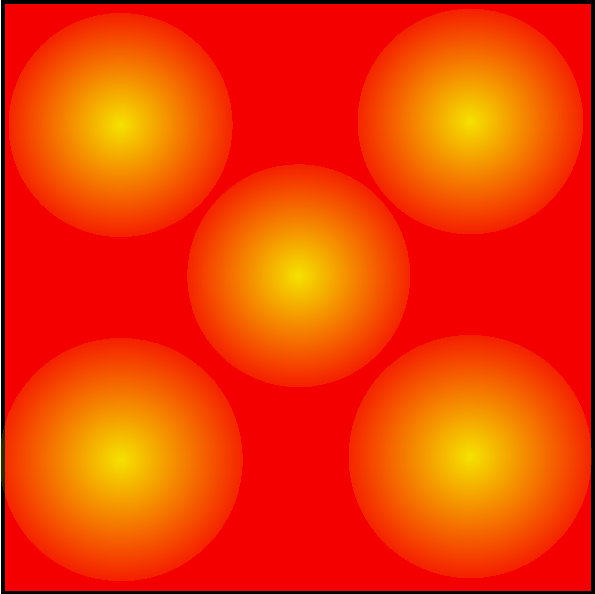
\includegraphics[width=\textwidth]{papers/swarm-intelligence2021/img/scenario/standard}
      \caption{}
      \label{fig:standard}
  \end{subfigure}
  \hfill
  \begin{subfigure}[b]{0.2\textwidth}
      \centering
      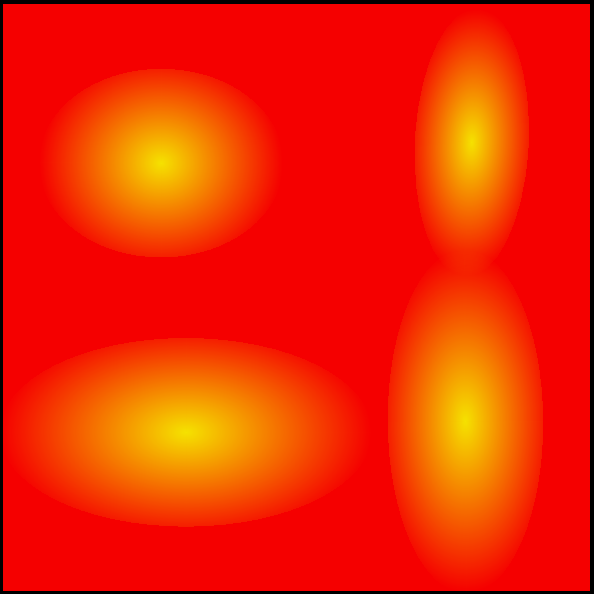
\includegraphics[width=\textwidth]{papers/swarm-intelligence2021/img/scenario/stretched}
      \caption{}
      \label{fig:stretched}
  \end{subfigure}
  \hfill
  \begin{subfigure}[b]{0.2\textwidth}
      \centering
      
\includegraphics[width=\textwidth]{papers/swarm-intelligence2021/img/scenario/one-direction.pdf}
      \caption{}
      \label{fig:one-direction}
  \end{subfigure}
  \\
  \centering
  \begin{subfigure}[b]{0.2\textwidth}
      \centering
      
\includegraphics[width=\textwidth]{papers/swarm-intelligence2021/img/scenario/one-direction-one-candidate.pdf}
      \caption{}
      \label{fig:one-direction-one-candidate}
  \end{subfigure}
  \hfill
  \begin{subfigure}[b]{0.2\textwidth}
      \centering
      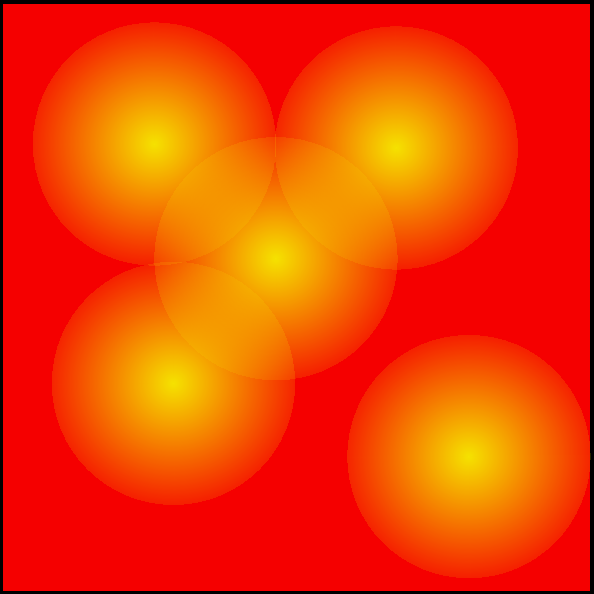
\includegraphics[width=\textwidth]{papers/swarm-intelligence2021/img/scenario/standard-overlay.pdf}
      \caption{}
      \label{fig:overlapped}
  \end{subfigure}
  \hfill
  \begin{subfigure}[b]{0.2\textwidth}
      \centering
      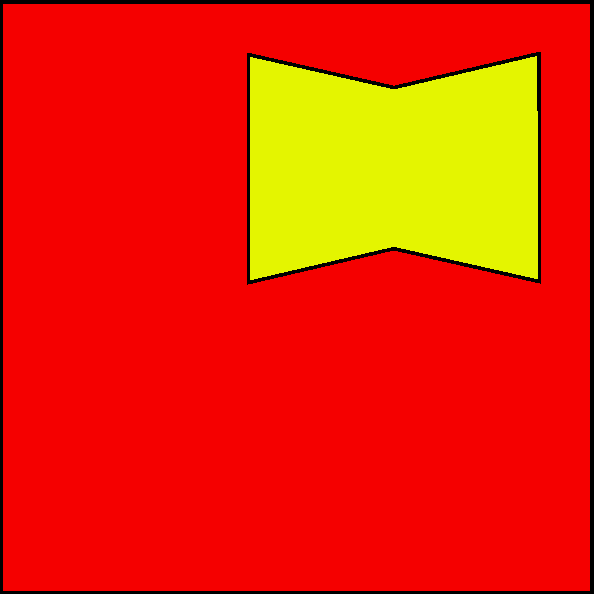
\includegraphics[width=\textwidth]{papers/swarm-intelligence2021/img/scenario/non-convex.pdf}
      \caption{}
      \label{fig:non-convex}
  \end{subfigure}
  \caption{Graphical representation of temperature field distributions used in the simulations. 
  The lighter the colour, the lower the temperature. }
  \label{fig:field-phenomena-distribution}
\end{figure}
\begin{figure}[t]
  \begin{subfigure}[b]{0.45\textwidth}
    \centering
    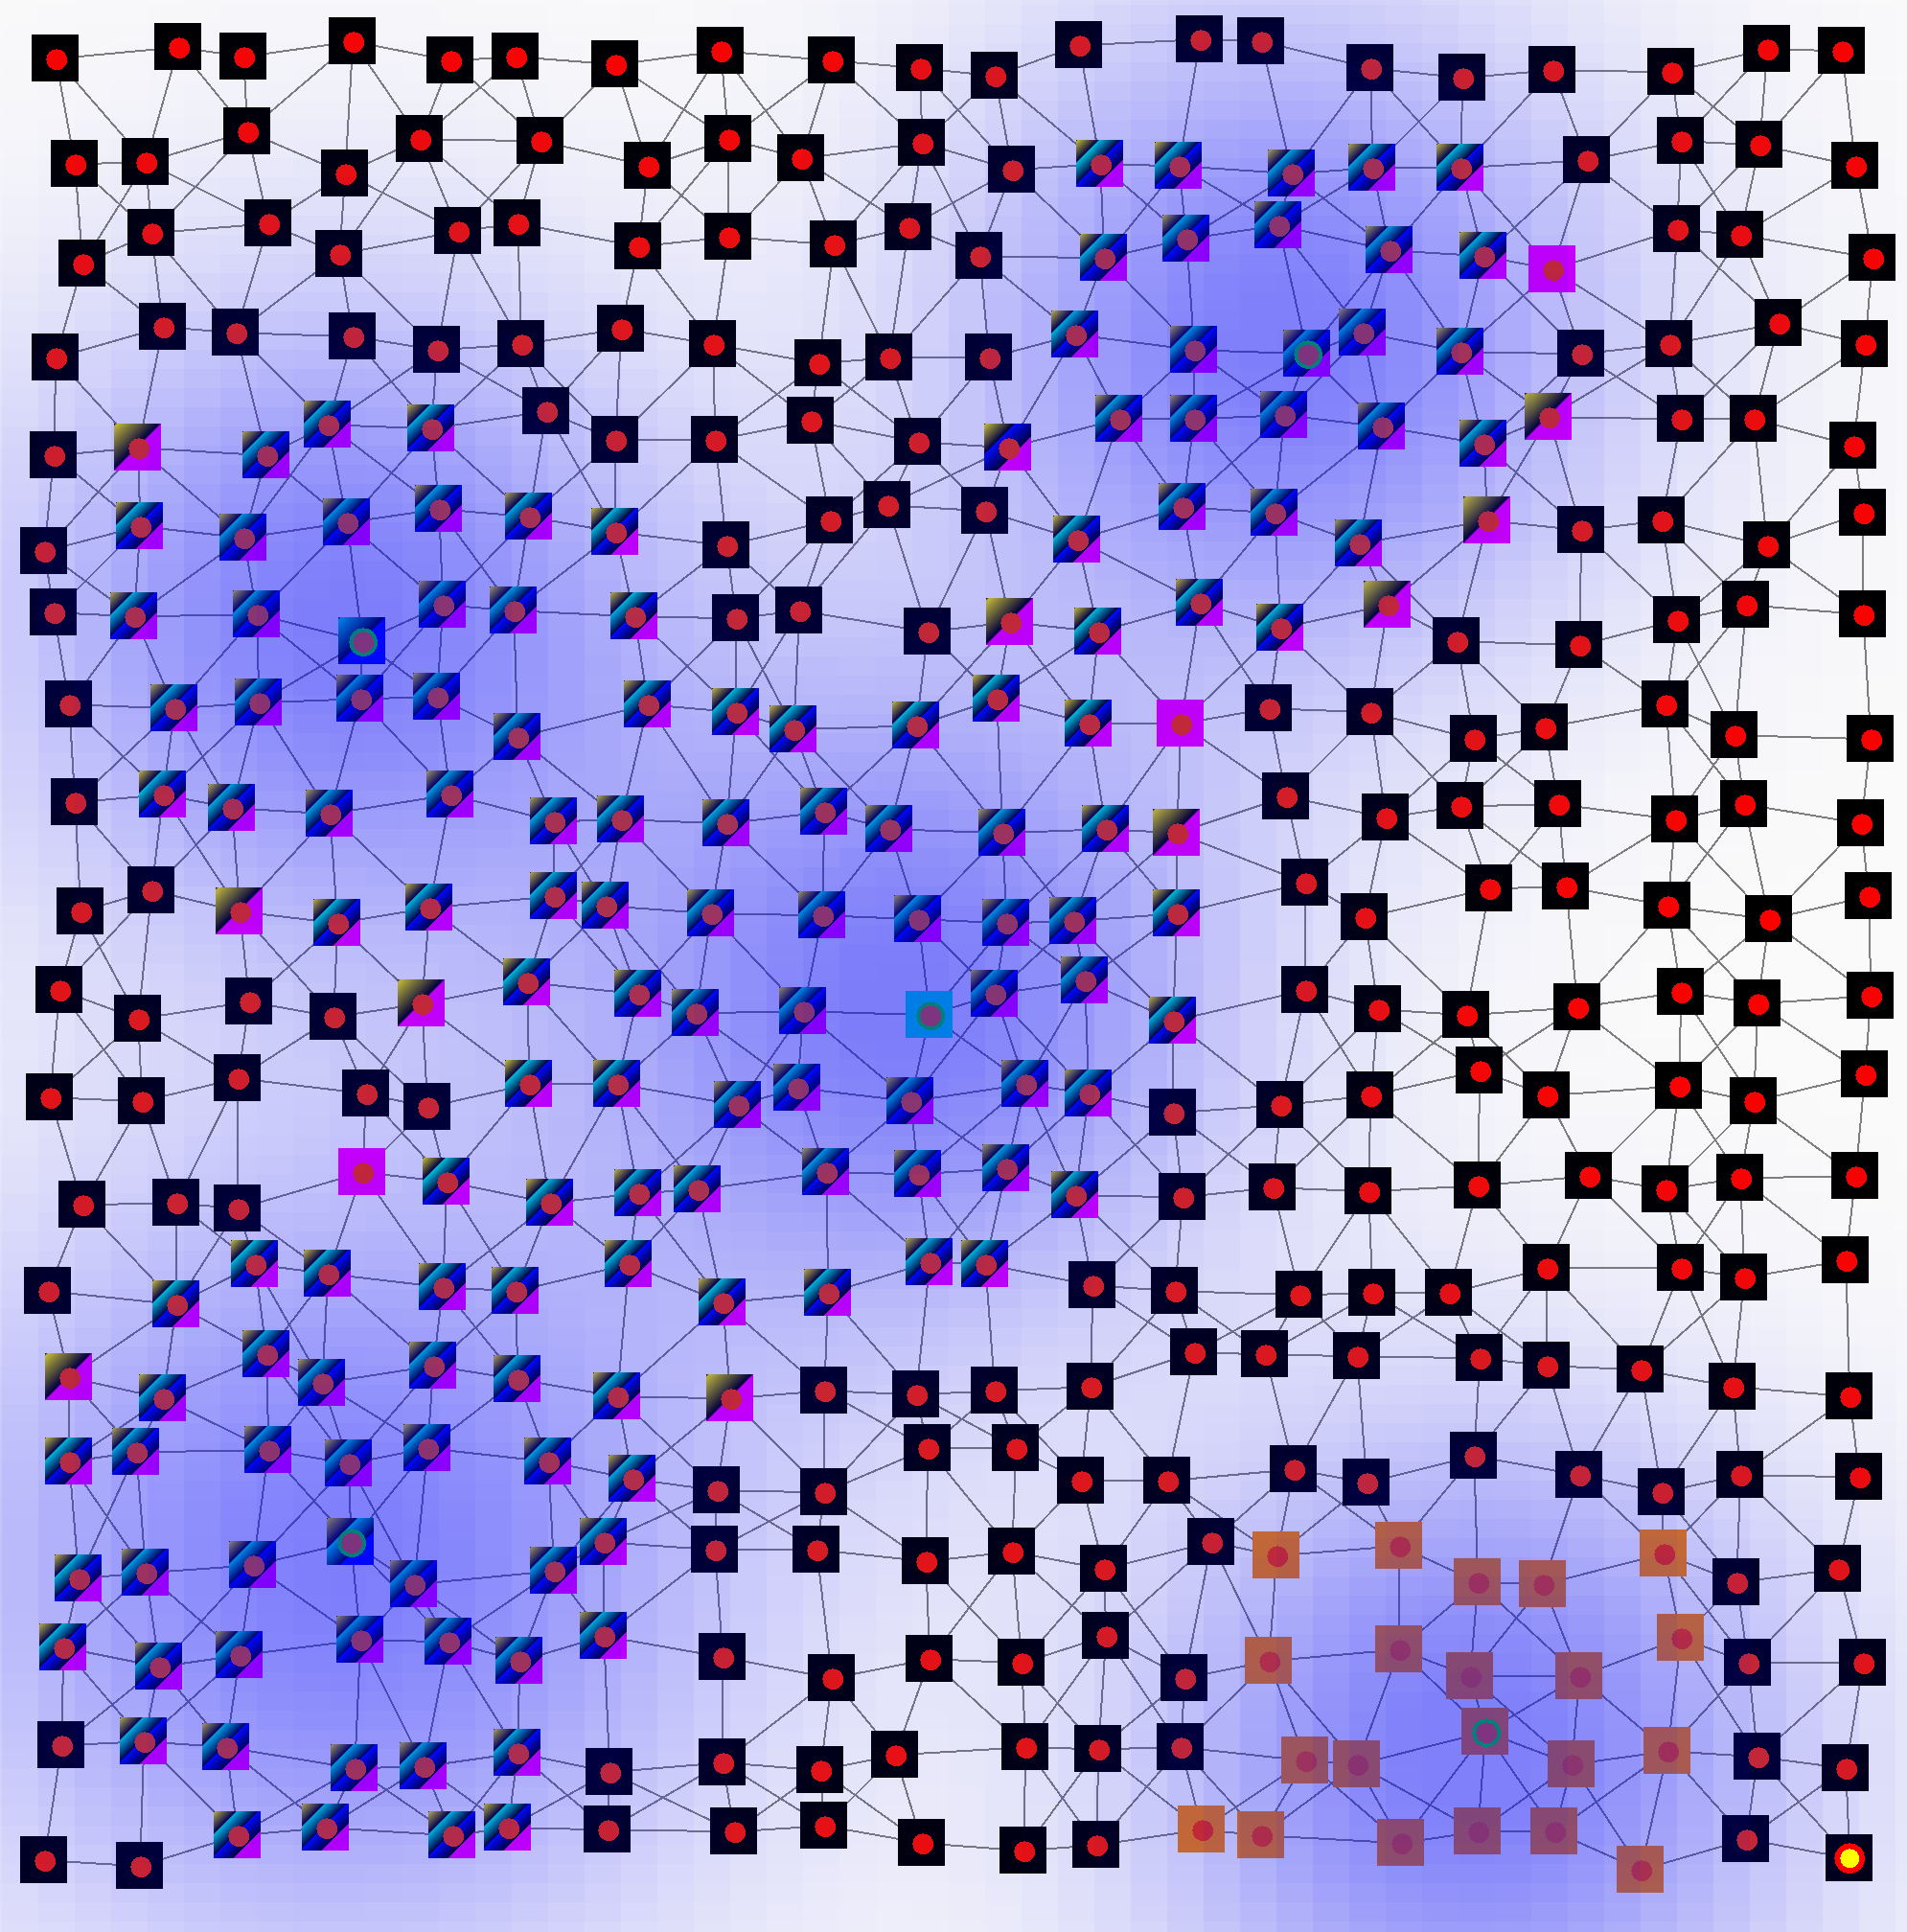
\includegraphics[width=\textwidth]{papers/swarm-intelligence2021/img/simulation-execution.png}
  \end{subfigure}
  \begin{subfigure}[b]{0.45\textwidth}
    \centering
    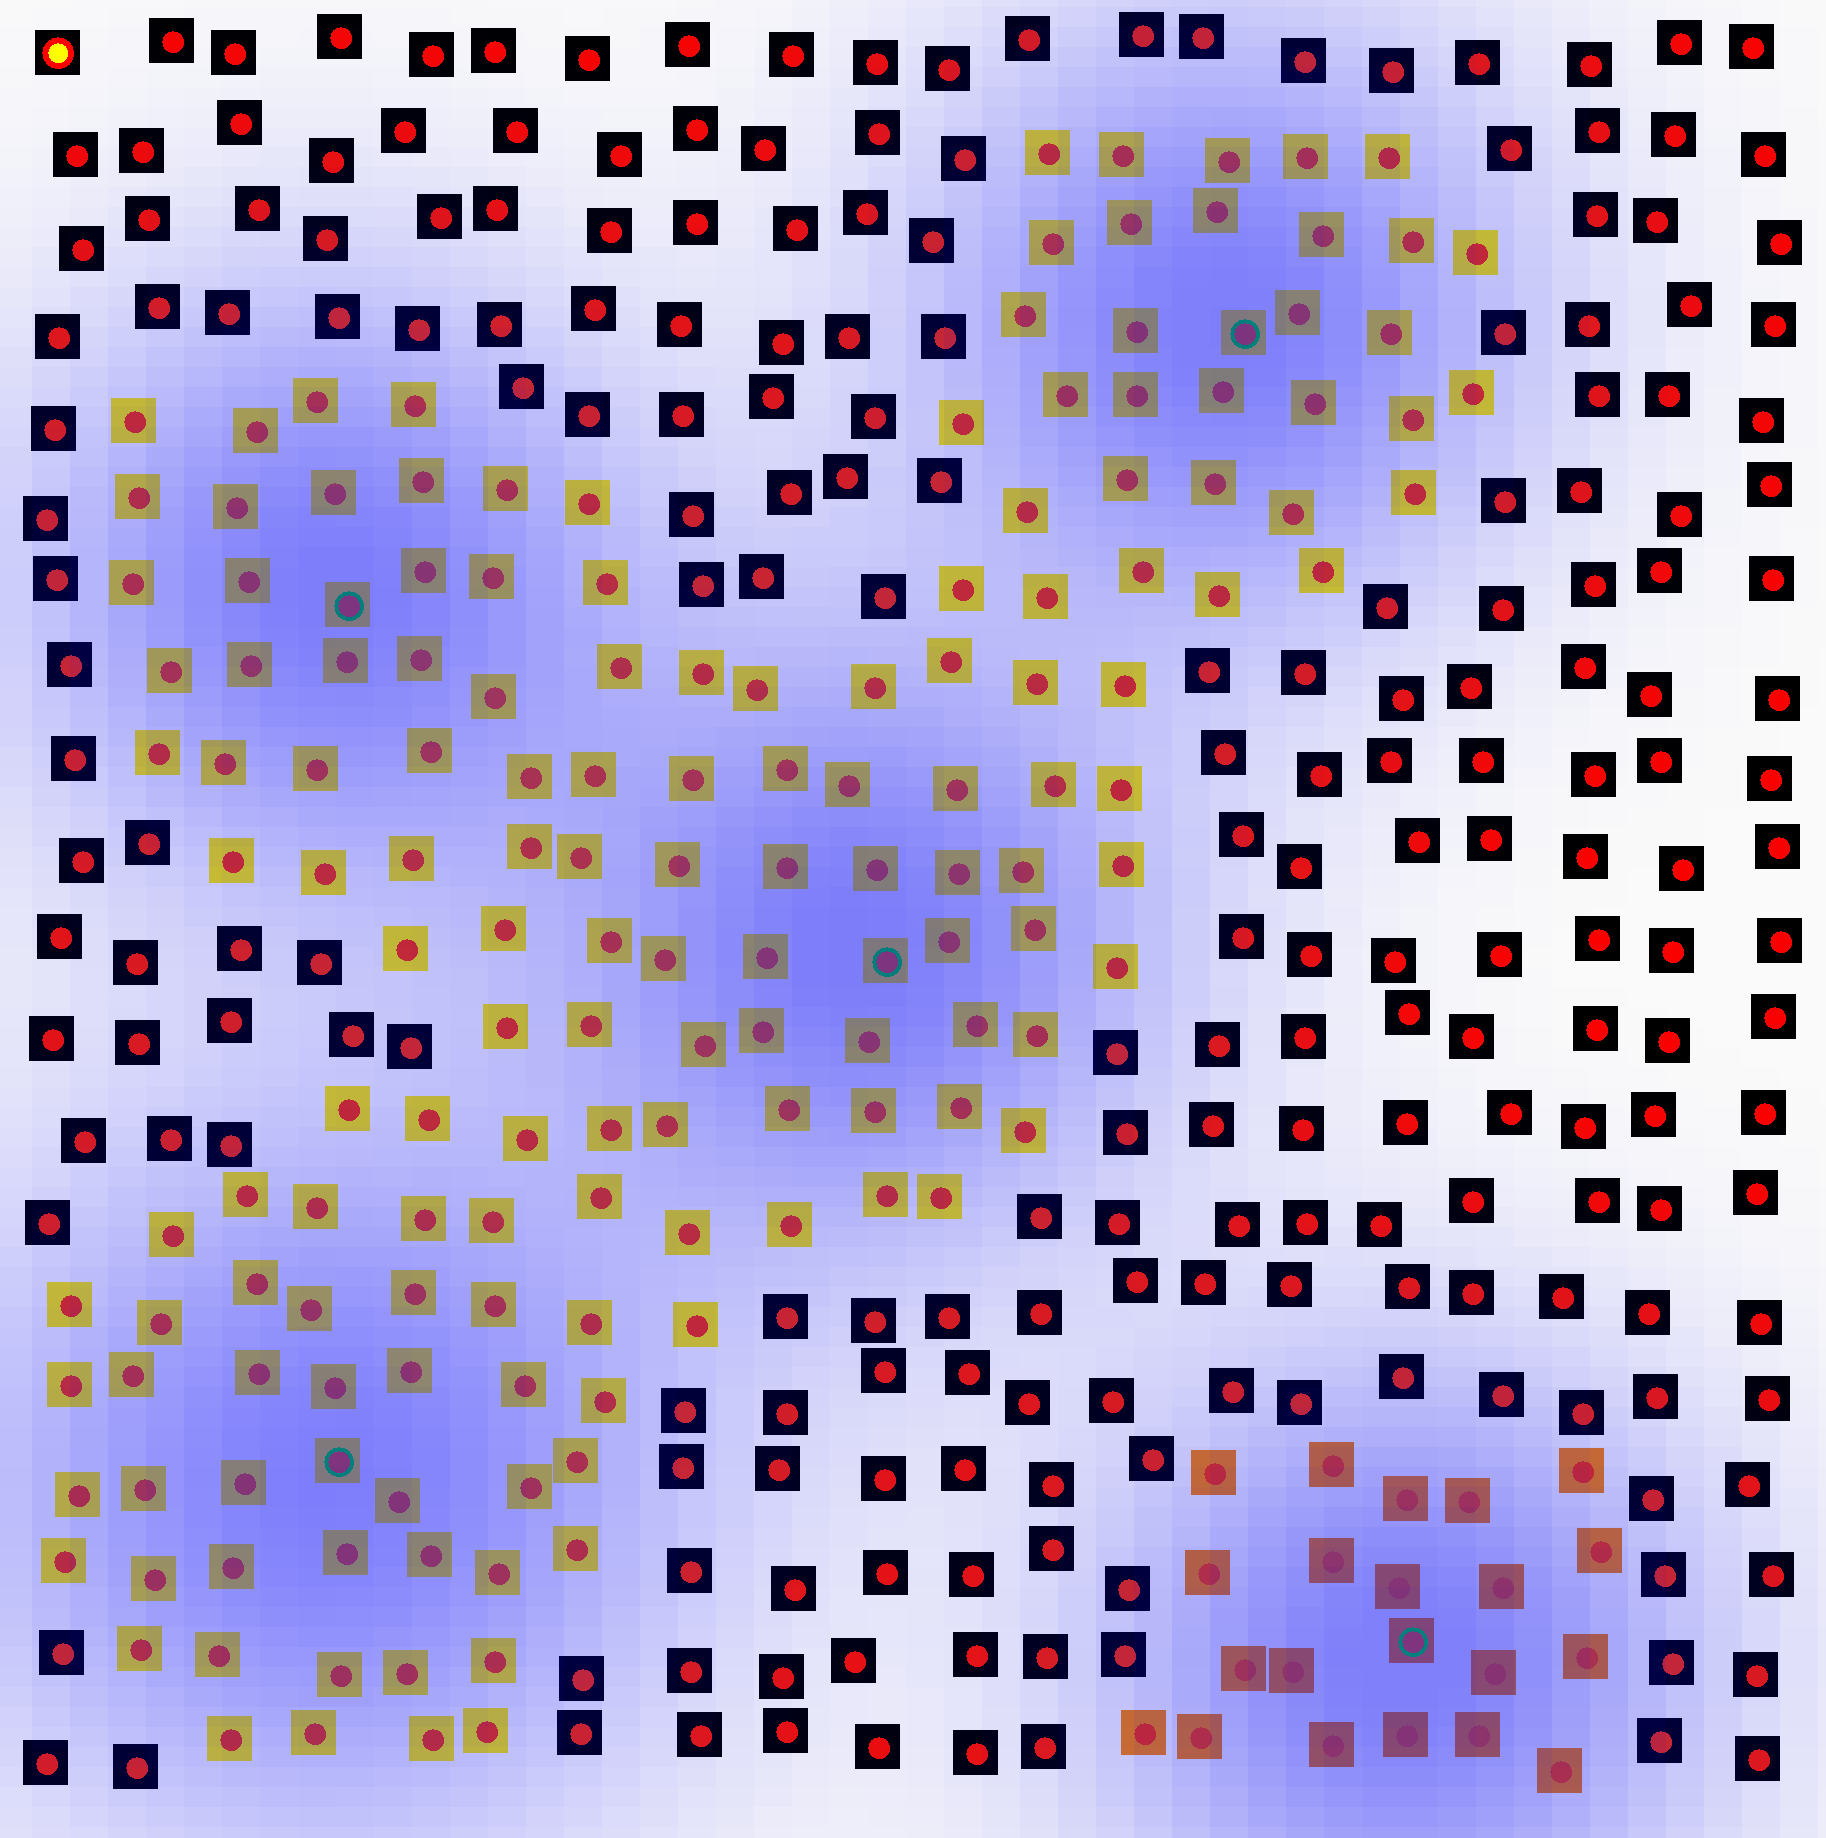
\includegraphics[width=\textwidth]{papers/swarm-intelligence2021/img/after-merge.png}
  \end{subfigure}
  \centering
  \caption[Snapshots of simulation executions during the sensing-driven clustering.]{Snapshots of simulation executions. 
  The colour of the square identifies the cluster ID found in that point. 
  Black colour means no cluster. 
  The green circle means that the node is a candidate. 
  The blue gradient circles are a graphical representation of temperature distribution. 
  On the left is shown a snapshot of a simulation before the merge policy has been applied (multiple clusters per point are found). 
  On the right, there is the snapshot of the same simulation after the merge policy action.}
  \label{fig:simulation-snapshot}
\end{figure}

We evaluate the behaviour of our algorithm in several experiments. %(explained below and illustrated in \Cref{fig:field-phenomena-distribution}).
 The simulations have in common
 \begin{enumerate*}%[i)]
  \item the environment area (a square with a side of 1km),
  \item the communication radius (\SI{100}{\metre}), and
  \item the average evaluation frequency of aggregate programs (\SI{1}{\hertz}).
\end{enumerate*}
The drones are uniformly placed to cover the entire zone.
We run the simulations in a modern machine equipped with two AMD EPYC 7301 with \SI{128}{\giga\byte} RAM.
 The results are reproducible in any modern machine, but consider that it might take a long time to finish
 (in our configuration, the simulations end after \SI{8}{\hour}).
%
Each scenario is executed 20 times with different random seeds
 for a total of 100 simulated seconds (some simulations lasts \SI{150}{\second} to reach convergence).
%
The selection of scenarios presented below aims to achieve two main objectives:
\begin{enumerate}
    \item assess the effectiveness of our algorithm,
    \item ensure that it meets all the previously outlined goals.
\end{enumerate}
Specifically, we chose scenarios where most temperature distributions follow a normal distribution. 
 This choice is grounded in the observation that natural phenomena often exhibit such distributions. 
 Consequently, if our algorithm succeeds in identifying clusters in these Gaussian scenarios, it is likely to be effective in other contexts where monitoring natural phenomena is essential. 
 To complement this, we also tested the algorithm's ability to identify non-Gaussian shapes, as evidenced in scenarios 3, 4, and 5.

The final set of scenarios is designed to evaluate the system's adaptability to changes at both the system level, 
 such as movement and failures, and the environmental level, like variations in distribution over time.

The simulation data is processed using NumPy~\cite{harris2020array} and visualized through matplotlib~\cite{Hunter:2007}.
%
The plotted results consist of the average (lines)
 and the standard deviation (area behind lines)
 of the values of interest in different episodes.
%
In \Cref{fig:simulation-snapshot} there is a graphical representation of a run of our algorithm.

\paragraph{Scenario 1: Gaussian patterns (\Cref{fig:standard})}
\subparagraph{Description}
In this scenario, the drones are stationary (i.e., they stand still).
 There are five zones with a Gaussian distribution, and there is no overlap between distributions.
 Given the stationary situation, the number of candidate nodes is equal to the number of zones of interest.

\subparagraph{Why} Used to verify \ref{goal:1}, particularly
 we expect that the algorithm finds clusters without making any errors and that they will be stable over time.
%%%%%%%%%%%%%%%%%%%%%%
\paragraph{Scenario 2: Stretched Gaussian patterns (\Cref{fig:stretched})}
\label{scenario-2}
\subparagraph{Description}
These simulations are similar to the previous one, but in this case, the Gaussian distributions have an ellipse-like shape.
\subparagraph{Why}
With these experiments, we would check that the shape does not make such a difference in the clustering process.
 Indeed, we expect a result similar to the one in the previous example (\ref{goal:1}).
%%%%%%%%%%%%%%%%%%%%%%
\paragraph{Scenario 3: One direction temperature field (\Cref{fig:one-direction,,fig:one-direction-one-candidate})}
\subparagraph{Description} In this case, we imagine that only one cluster is present
 (fixing $\theta$ to \SI{1}{\celsius} and putting a total variation of temperature equal to \SI{1}{\celsius}).
 Temperatures grow from left to right in a constant fashion. \rev{Namely, in \Cref{fig:one-direction} the temperature varies in one dimension (horizontally), whereas in \Cref{fig:one-direction-one-candidate} the temperature varies in two dimensions (diagonally)}.
\rev{In the scenario depicted in \Cref{fig:one-direction}} we are interested to see what happens when multiple candidates are elected.
 In this case, there are several relative minima (the set of nodes that are leftmost with minimum ID in their neighbourhood).
 But, eventually, the processes will expand them in the same way.
 Thus, we expect that the merging policy tends to create only one cluster.
 We use the scenario shown in \Cref{fig:one-direction-one-candidate} as a reference.
Indeed, there will be only one candidate (located in the bottom left corner),
and hence the algorithm should result in one cluster.
\subparagraph{Why} We devise these experiments to test the effectiveness of the merging policy and to verify the goal \ref{goal:1}.


%%%%%%%%%%%%%%%%%%%%%%
\paragraph{Scenario 4: Gaussian overlapped patterns (\Cref{fig:overlapped})}
\subparagraph{Description}
In this case, we have several Gaussian patterns that could be overlapped. We imagine that the $\theta$ value is essential here:
 if the value is too high, the system will recognise the set of overlapping clusters as one;
 otherwise, it will consider disjointed.
\subparagraph{Why}
This experiment serves to emphasize that $\theta$ is a domain-dependent choice.
 Moreover, it will show that the algorithm could be used also to find overlapped situations (\ref{goal:1}).
\paragraph{Scenario 5: Non convex patterns (\Cref{fig:non-convex})}
\subparagraph{Description}
 In this case, there are two zones, one with a non-convex shape with a lower temperature than the outer zone.
 Here we expect that, eventually, the system will identify the presence of only two clusters.
 The program might identify several candidates in the transitory phases (cf. one for each edge).
 Hence, the merging policy should fix this issue by producing only two clusters.
 \subparagraph{Why} With this scenario, we want to point out that the program can cope with zones of arbitrary shape.
\paragraph{Scenario 6: Gaussian patterns with movement}
\subparagraph{Description}
We test the result using four Gaussian distributions (arranged similarly to \Cref{fig:standard}) combined with movement.
 Here, both merging policy, and \emph{waiting candidate time} ($\beta$) will be essential.
 In particular, $\beta$ helps to avoid false positives since it waits before spawning a new clustering process when encounters small local temperature variations.
 In general, we imagine that high values of $\omega$ and $\zeta$ will make the algorithm more unstable.
\subparagraph{Why} We are interested in seeing how movement affects the result of the clustering process (\ref{goal:2}).

\paragraph{Scenario 7: Variable size Gaussian pattern}
\subparagraph{Description}
In this experiment, the temperature distributions are placed similarly as \Cref{fig:standard},
 but then the size of areas evolves in time.
 We expand the areas until a time T and then contract them to their initial size.
 The starting area range is \SI{100}{\metre}, and the maximum area expansion is \SI{1}{\kilo\metre}.
 Here we expect that the cluster area follows the underlying temperature distribution.
\subparagraph{Why} In this experiment, we verify the algorithm's robustness against temperature changes (\ref{goal:3}).
\rev{
\paragraph{Scenario 8: Random Failures}
\subparagraph{Description}
 The temperature distribution of choice follows the \Cref{fig:standard}.
Nodes could disappear randomly with a rate specified by \emph{failure frequency}.
 This could be harmful when: i) the failure happens in a leader node,
  and therefore the cluster formed should be destroyed and, ii) the failures are so frequent that
  certain nodes became isolated.
  The second case is avoided using \emph{spawn frequency}, which forces the system to insert a new node
  with the specified rate.
In this case, we expect robust performance with high-density system (i.e., $\alpha$ = 0.5) since
 spurious failure does not change the overall topology.
\subparagraph{Why} In this last scenario, we check how the system handles node failures during the clustering process (\ref{goal:3}).
}
\subsection{Results}\label{s:eval:results}
\begin{figure}[t]
  %%% Scenario 1 %%%
  \centering
  \begin{subfigure}[b]{0.32\textwidth}
    \centering
    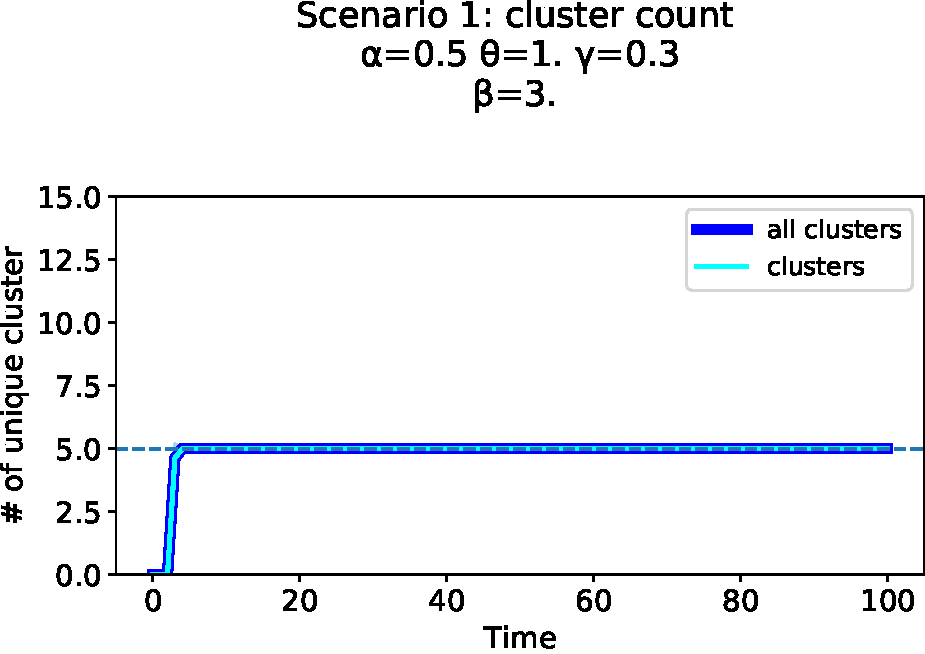
\includegraphics[width=\textwidth]{papers/swarm-intelligence2021/img/simulations/standard_cluster_count.pdf}
  \end{subfigure}
  \hfill
  \centering
  %%% Scenario 2 %%%
  \begin{subfigure}[b]{0.32\textwidth}
    \centering
    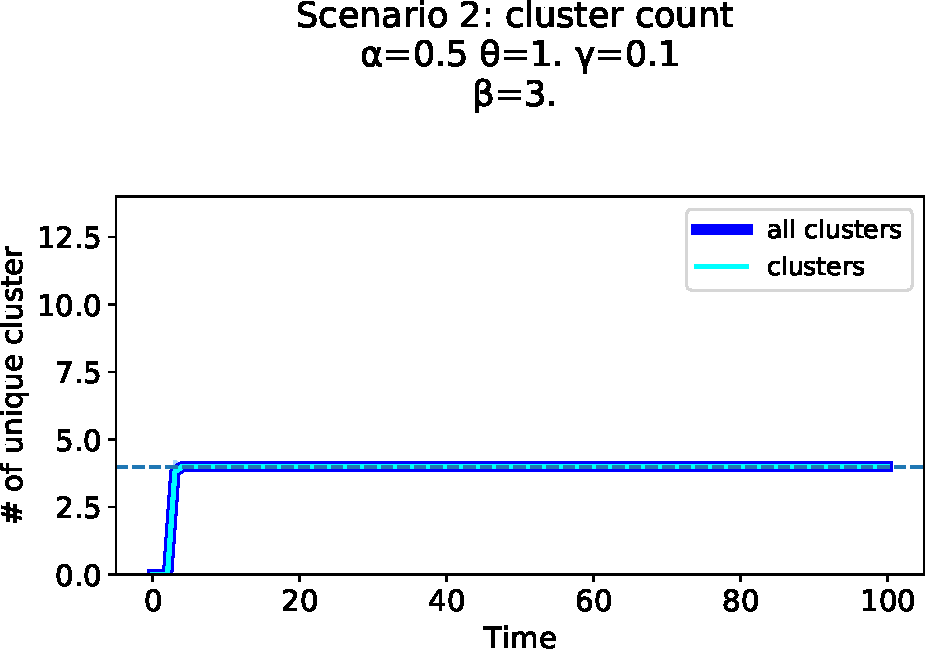
\includegraphics[width=\textwidth]{papers/swarm-intelligence2021/img/simulations/stretched_cluster_count.pdf}
  \end{subfigure}
  \hfill
  \centering
  %%% Scenario 3 %%%
  \begin{subfigure}[b]{0.32\textwidth}
    \centering
    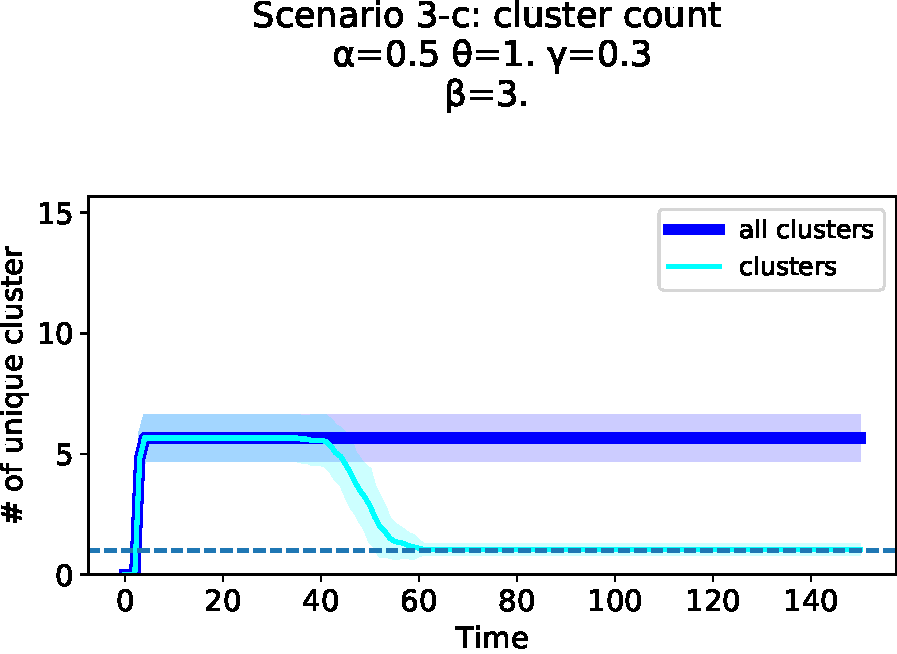
\includegraphics[width=\textwidth]{papers/swarm-intelligence2021/img/simulations/one-direction_0_021_α-0.5_θ-1._γ-0.3_β-3._ω-0._ζ-0..pdf}
  \end{subfigure}
  \hfill
  \centering
  %%% Scenario 4 %%%
  \begin{subfigure}[b]{0.32\textwidth}
    \centering
    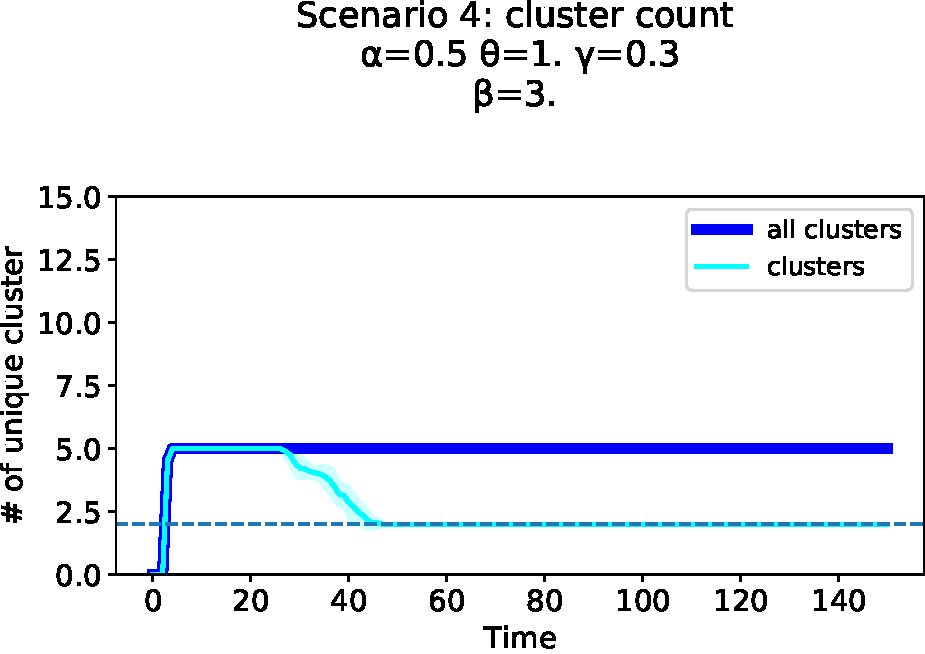
\includegraphics[width=\textwidth]{papers/swarm-intelligence2021/img/simulations/overlay_0_021_α-0.5_θ-1._γ-0.3_β-3._ω-0._ζ-0..pdf}
  \end{subfigure}
  \hfill
  \centering
  %%% Scenario 5 %%%
  \begin{subfigure}[b]{0.32\textwidth}
    \centering
    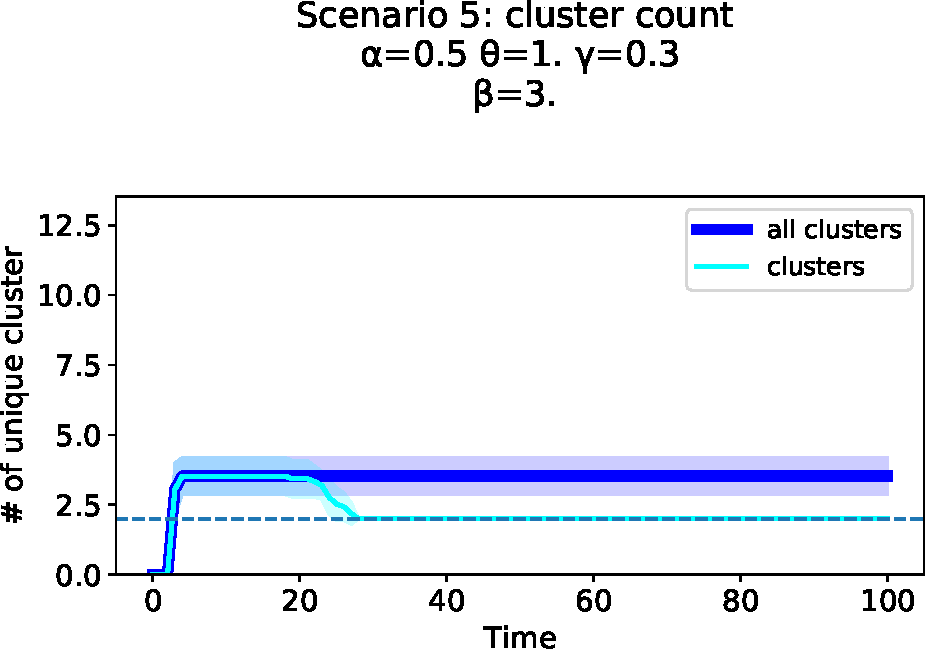
\includegraphics[width=\textwidth]{papers/swarm-intelligence2021/img/simulations/non-convex_0_021_α-0.5_θ-1._γ-0.3_β-3._ω-0._ζ-0..pdf}
  \end{subfigure}
  \hfill
  \centering
  %%% Scenario 6 %%%
  \begin{subfigure}[b]{0.32\textwidth}
    \centering
    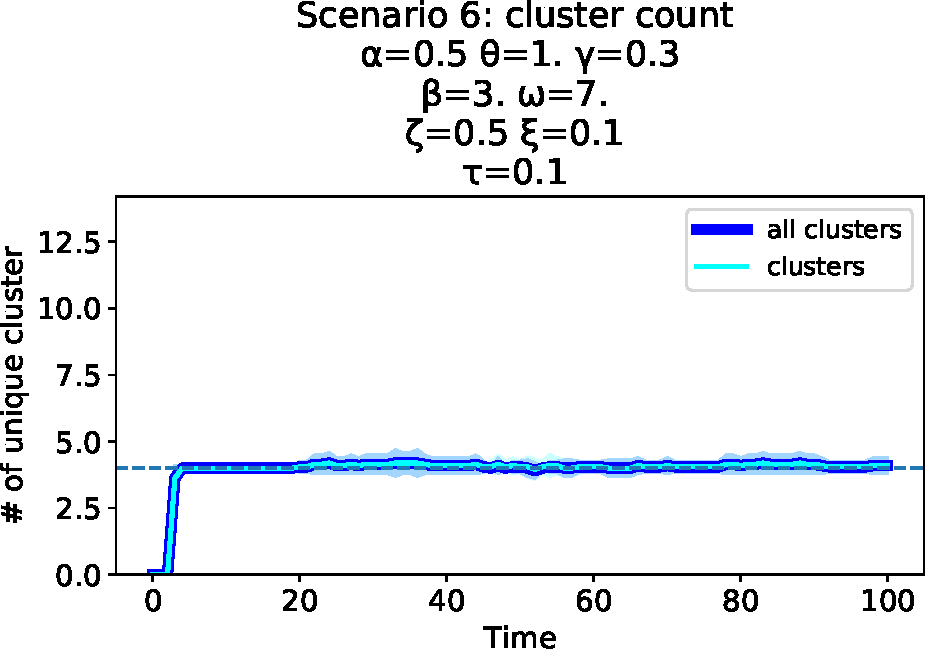
\includegraphics[width=\textwidth]{papers/swarm-intelligence2021/img/simulations/movement_cluster_count.pdf}
  \end{subfigure}
  \centering
  %%% Scenario 7 %%%
  \begin{subfigure}[b]{0.32\textwidth}
    \centering
    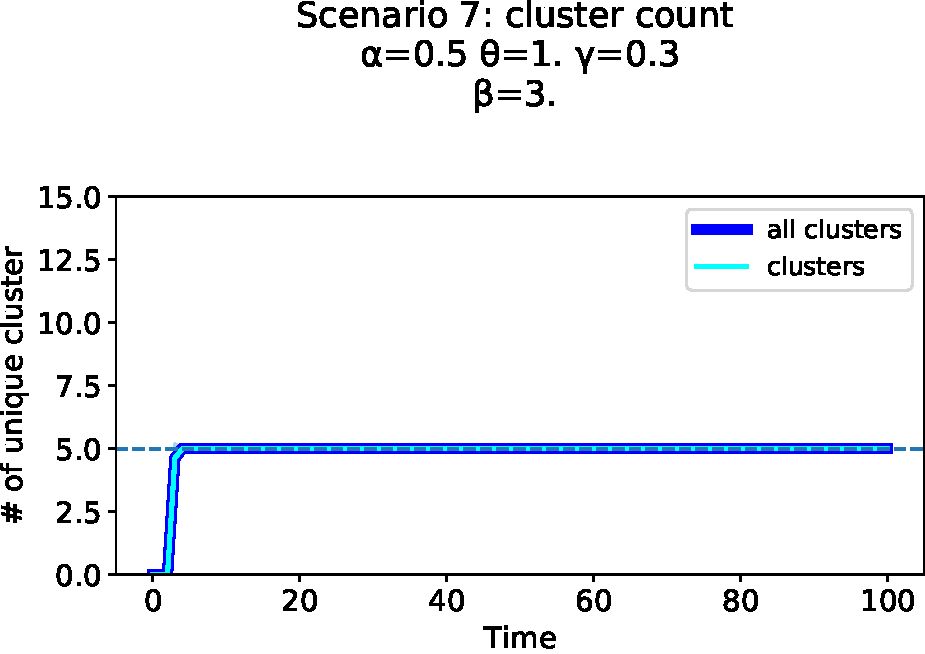
\includegraphics[width=\textwidth]{papers/swarm-intelligence2021/img/simulations/standard-updatable_0_021_α-0.5_θ-1._γ-0.3_β-3._ω-0._ζ-0..pdf}
  \end{subfigure}
  %%% Scenario 8 %%%
  \begin{subfigure}[b]{0.32\textwidth}
    \centering
    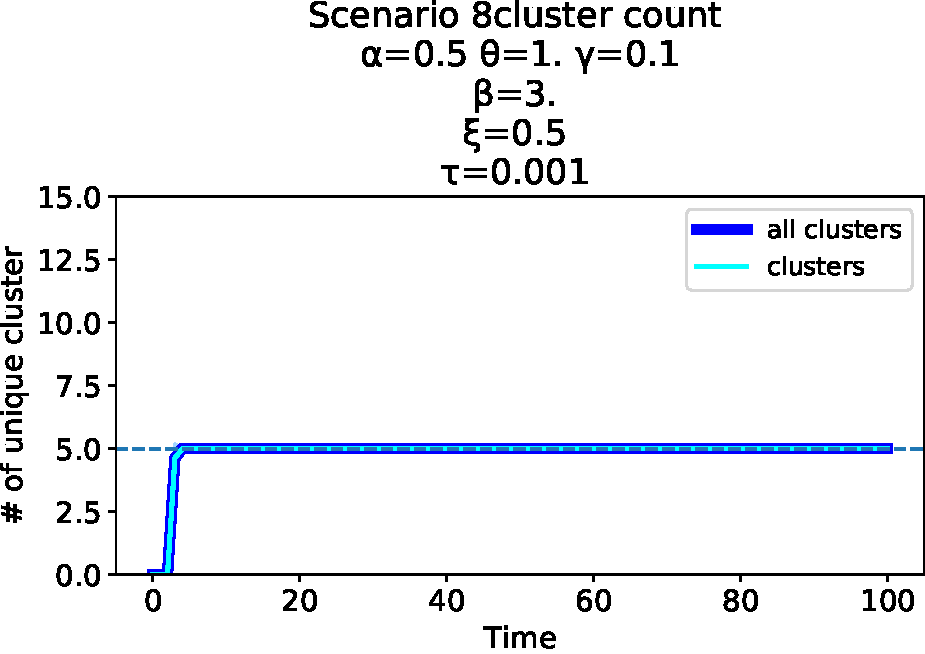
\includegraphics[width=\textwidth]{papers/swarm-intelligence2021/img/simulations/failScenario_0_021_α-0.5_θ-1._γ-0.1_β-3._ω-0._ζ-0._ξ-0.5_τ-0.001}
  \end{subfigure}
  \caption[Overview of simulation results in different clustering scenarios]{Overview of simulation results. 
  The dotted lines identify the ideal cluster division count. 
  The blue lines show the unique cluster found. 
  Instead, the cyan lines indicate the unique cluster number after the merging phase. 
  %In each scenario, the algorithm eventually reaches the correct cluster division count. 
  }
  \label{fig:overview-results}
\end{figure}
\begin{figure}[!ht]
  \begin{subfigure}[b]{0.32\textwidth}
    \centering
    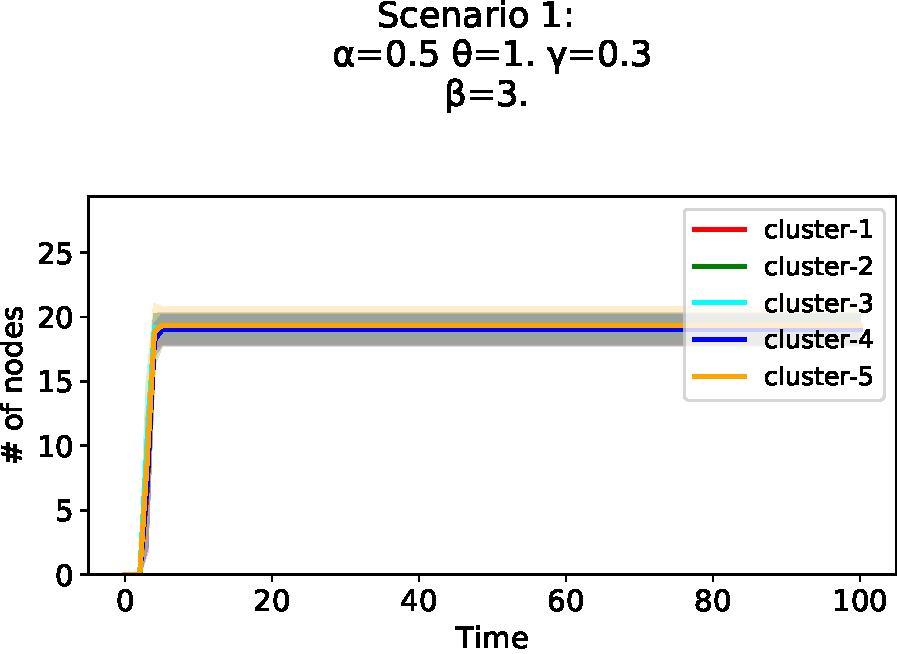
\includegraphics[width=\textwidth]{papers/swarm-intelligence2021/img/simulations/standard-count_0_034567_α-0.5_θ-1._γ-0.3_β-3._ω-0._ζ-0..pdf}
  \end{subfigure}
  \hfill
  \begin{subfigure}[b]{0.32\textwidth}
    \centering
    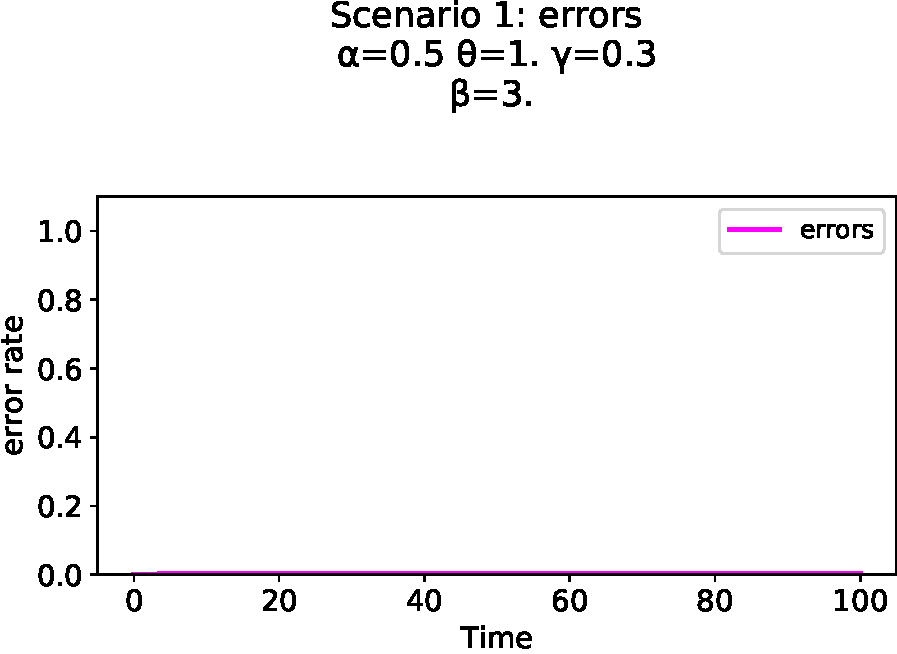
\includegraphics[width=\textwidth]{papers/swarm-intelligence2021/img/simulations/standard-errors_0_08_α-0.5_θ-1._γ-0.3_β-3._ω-0._ζ-0..pdf}
  \end{subfigure}
  \hfill
  \begin{subfigure}[b]{0.32\textwidth}
    \centering
    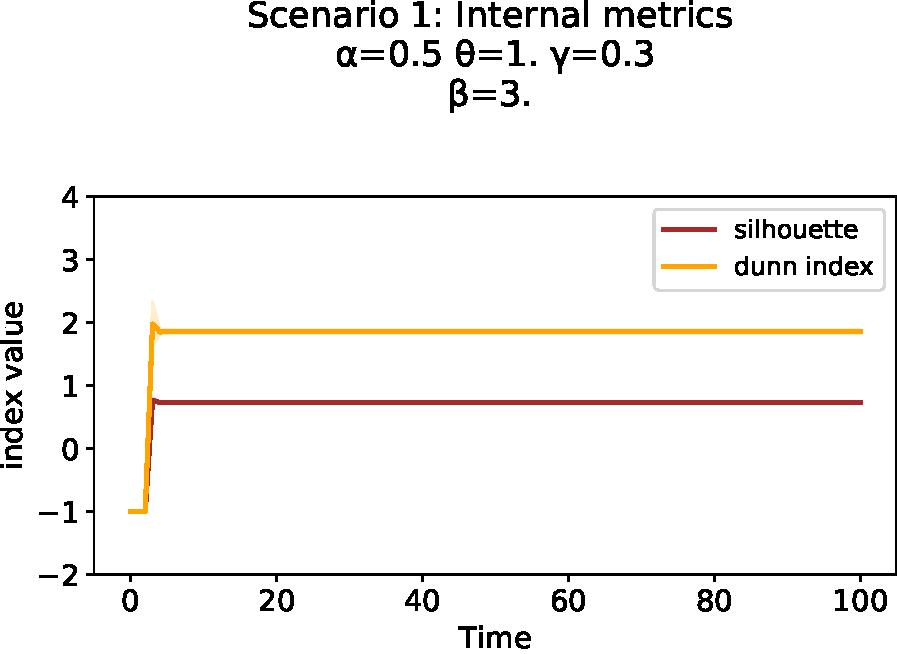
\includegraphics[width=\textwidth]{papers/swarm-intelligence2021/img/simulations/standard-metrics_0_0910_α-0.5_θ-1._γ-0.3_β-3._ω-0._ζ-0..pdf}
  \end{subfigure}
  \\
  \begin{subfigure}[b]{0.32\textwidth}
    \centering
    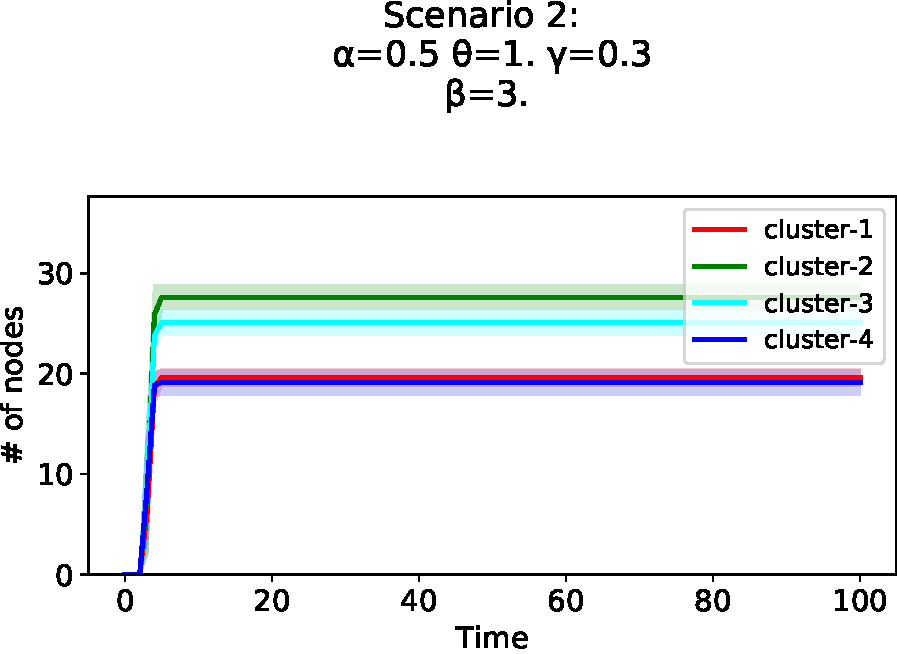
\includegraphics[width=\textwidth]{papers/swarm-intelligence2021/img/simulations/stretched-count_0_03456_α-0.5_θ-1._γ-0.3_β-3._ω-0._ζ-0..pdf}
  \end{subfigure}
  \hfill
  \begin{subfigure}[b]{0.32\textwidth}
    \centering
    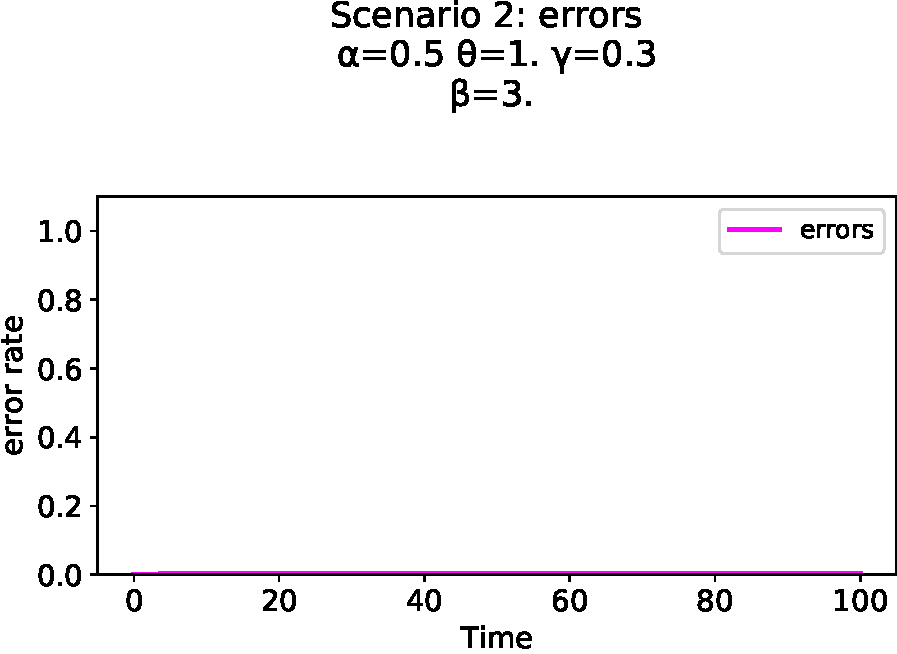
\includegraphics[width=\textwidth]{papers/swarm-intelligence2021/img/simulations/stretched-errors_0_08_α-0.5_θ-1._γ-0.3_β-3._ω-0._ζ-0..pdf}
  \end{subfigure}
  \hfill
  \begin{subfigure}[b]{0.32\textwidth}
    \centering
    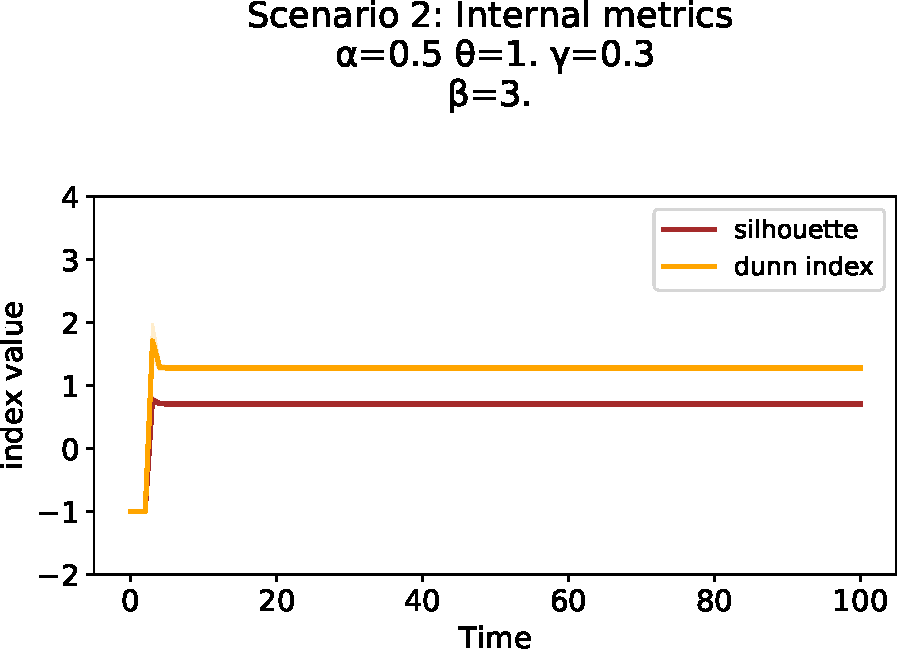
\includegraphics[width=\textwidth]{papers/swarm-intelligence2021/img/simulations/stretched-metrics_0_0910_α-0.5_θ-1._γ-0.3_β-3._ω-0._ζ-0..pdf}
  \end{subfigure}
  \\
  \begin{subfigure}[b]{0.32\textwidth}
    \centering
    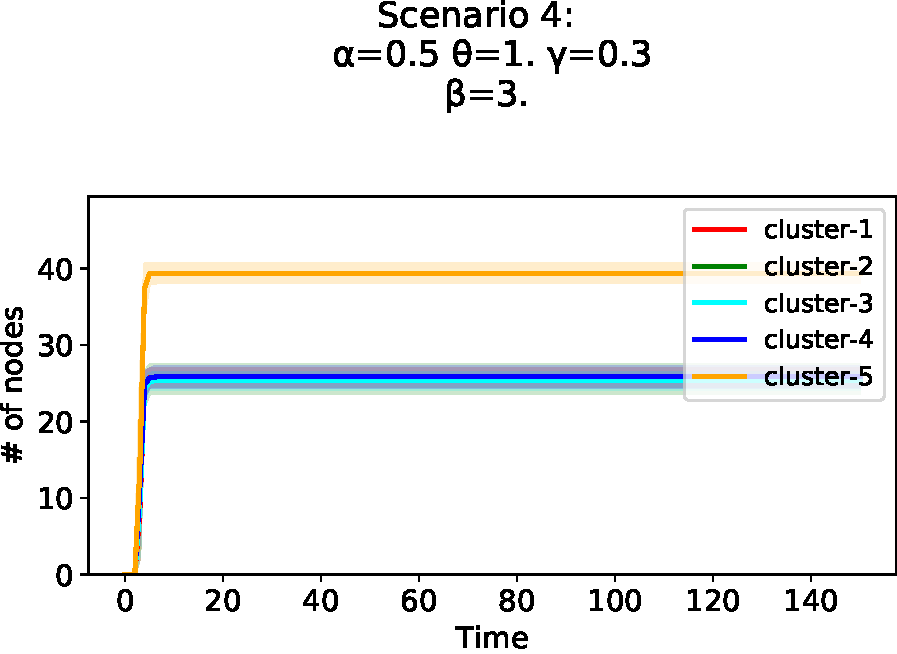
\includegraphics[width=\textwidth]{papers/swarm-intelligence2021/img/simulations/overlay-count_0_034567_α-0.5_θ-1._γ-0.3_β-3._ω-0._ζ-0..pdf}
  \end{subfigure}
  \hfill
  \begin{subfigure}[b]{0.32\textwidth}
    \centering
    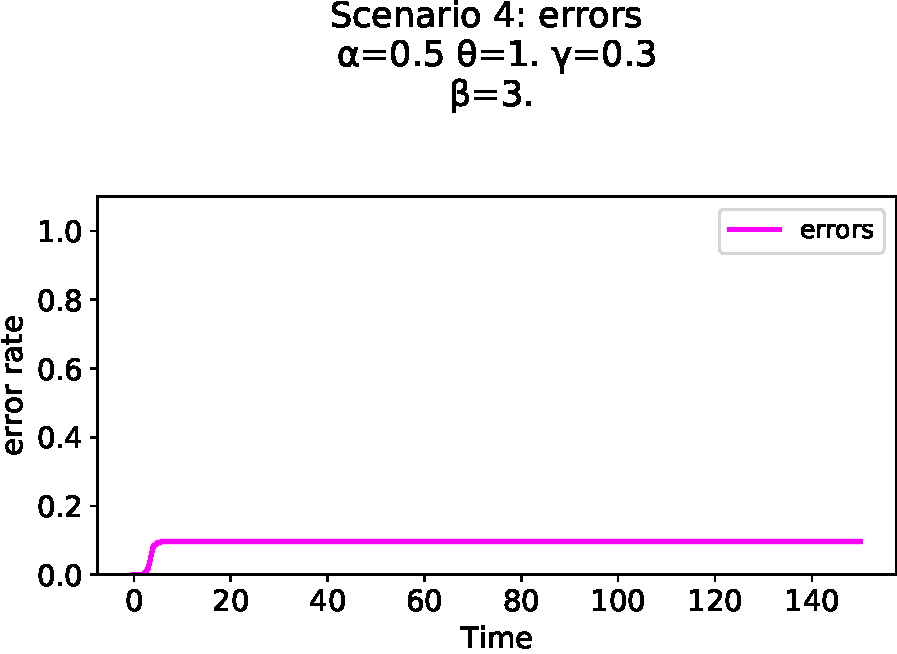
\includegraphics[width=\textwidth]{papers/swarm-intelligence2021/img/simulations/overlay-errors_0_08_α-0.5_θ-1._γ-0.3_β-3._ω-0._ζ-0..pdf}
  \end{subfigure}
  \hfill
  \begin{subfigure}[b]{0.32\textwidth}
    \centering
    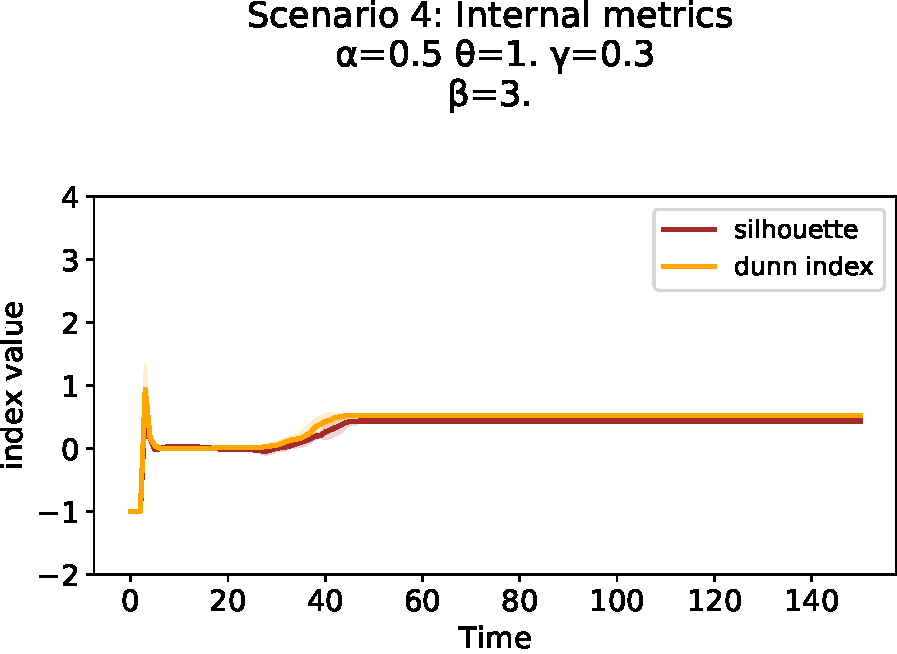
\includegraphics[width=\textwidth]{papers/swarm-intelligence2021/img/simulations/overlay-metrics_0_0910_α-0.5_θ-1._γ-0.3_β-3._ω-0._ζ-0..pdf}
  \end{subfigure}
  \\
  \begin{subfigure}[b]{0.32\textwidth}
    \centering
    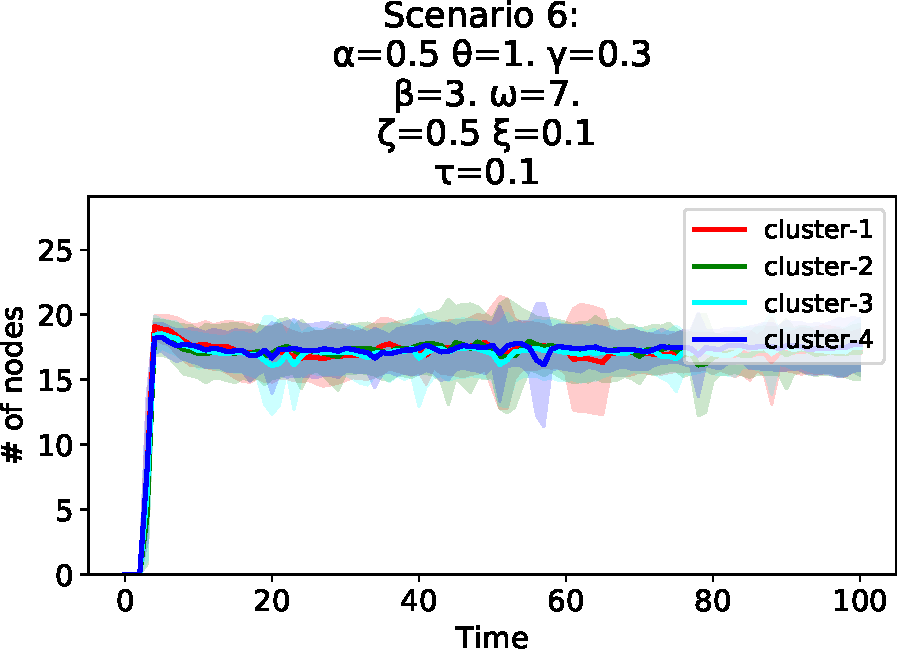
\includegraphics[width=\textwidth]{papers/swarm-intelligence2021/img/simulations/movement-count_0_03456_α-0.5_θ-1._γ-0.3_β-3._ω-7._ζ-0.5.pdf}
  \end{subfigure}
  \hfill
  \begin{subfigure}[b]{0.32\textwidth}
    \centering
    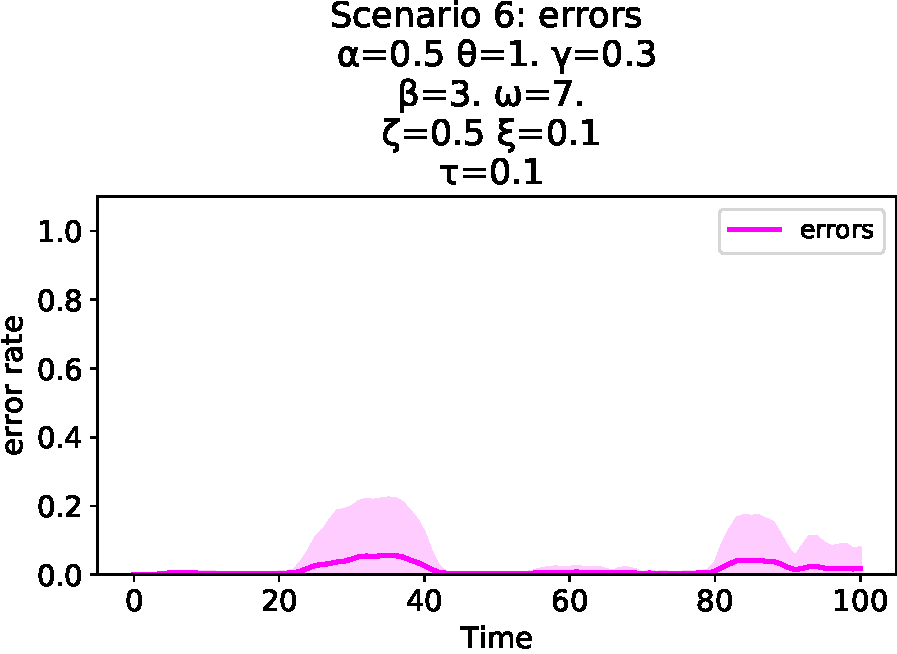
\includegraphics[width=\textwidth]{papers/swarm-intelligence2021/img/simulations/movement-errors_0_08_α-0.5_θ-1._γ-0.3_β-3._ω-7._ζ-0.5.pdf}
  \end{subfigure}
  \hfill
  \begin{subfigure}[b]{0.32\textwidth}
    \centering
    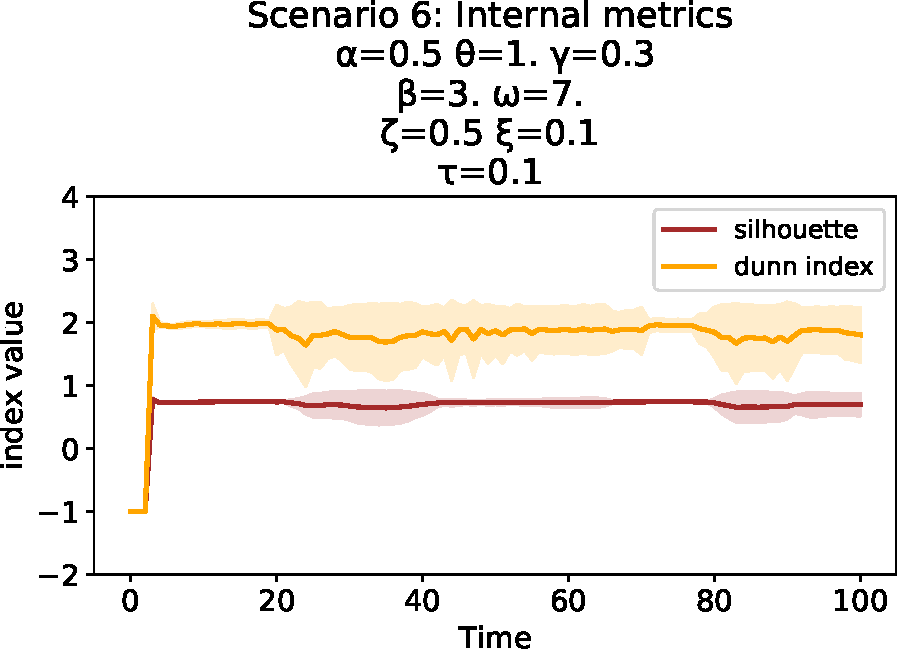
\includegraphics[width=\textwidth]{papers/swarm-intelligence2021/img/simulations/movement-metrics_0_0910_α-0.5_θ-1._γ-0.3_β-3._ω-7._ζ-0.5.pdf}
  \end{subfigure}
  \\
  \begin{subfigure}[b]{0.32\textwidth}
    \centering
    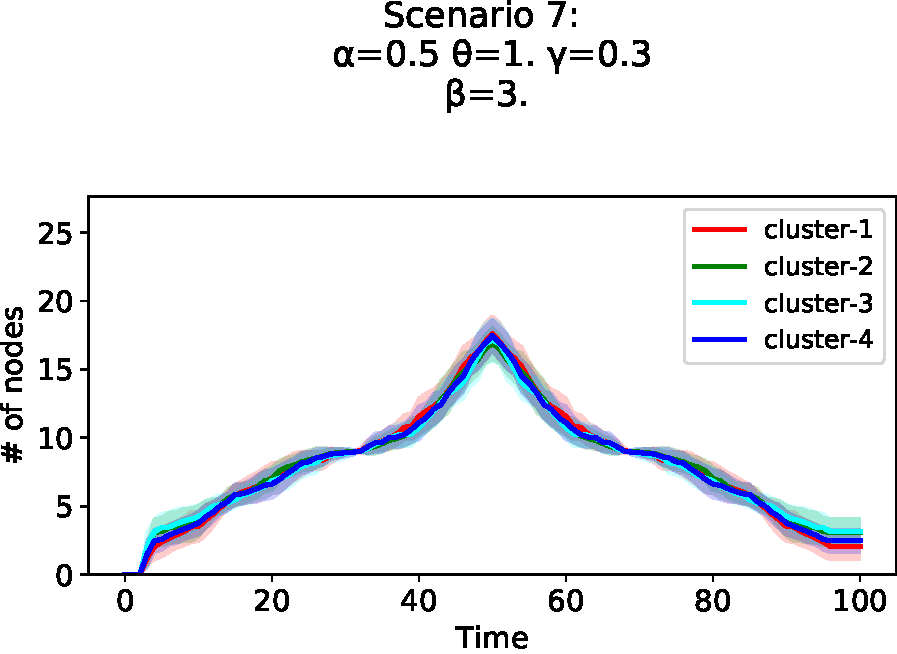
\includegraphics[width=\textwidth]{papers/swarm-intelligence2021/img/simulations/standard-updatable-count_0_03456_α-0.5_θ-1._γ-0.3_β-3._ω-0._ζ-0..pdf}
  \end{subfigure}
  \hfill
  \begin{subfigure}[b]{0.32\textwidth}
    \centering
    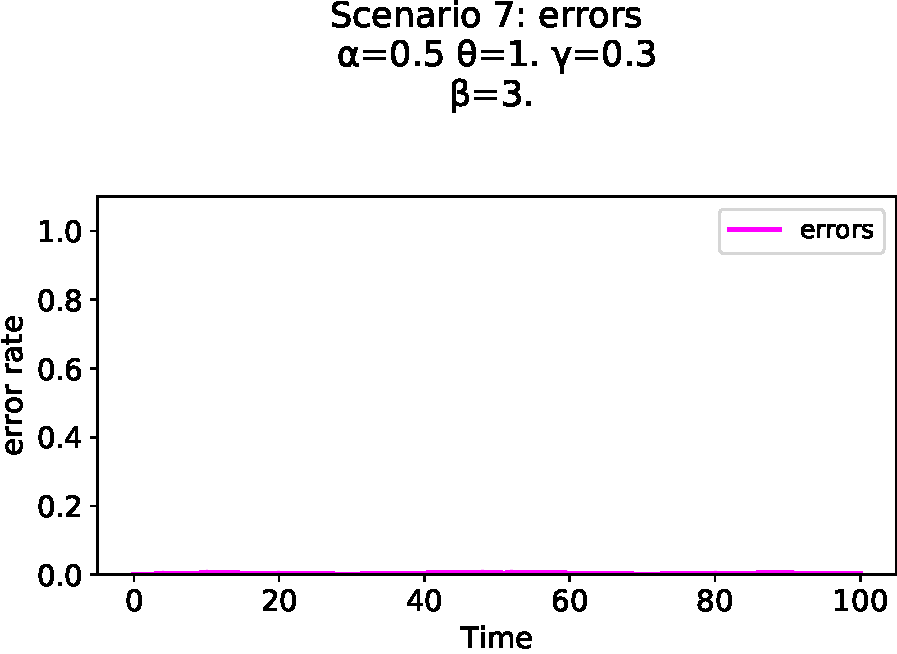
\includegraphics[width=\textwidth]{papers/swarm-intelligence2021/img/simulations/standard-updatable-errors_0_08_α-0.5_θ-1._γ-0.3_β-3._ω-0._ζ-0..pdf}
  \end{subfigure}
  \hfill
  \begin{subfigure}[b]{0.32\textwidth}
    \centering
    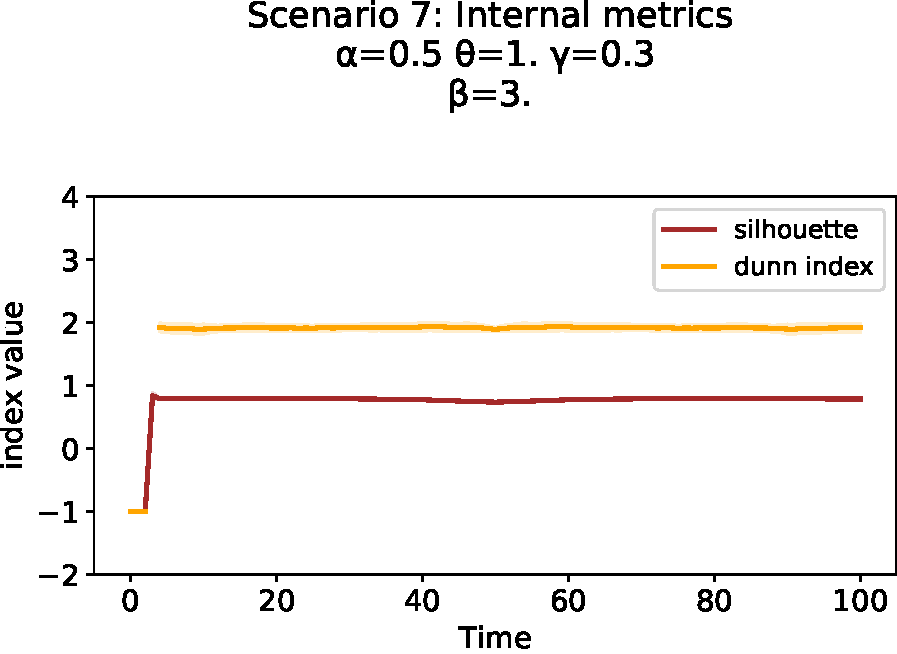
\includegraphics[width=\textwidth]{papers/swarm-intelligence2021/img/simulations/standard-updatable-metrics_0_0910_α-0.5_θ-1._γ-0.3_β-3._ω-0._ζ-0..pdf}
  \end{subfigure}
  \\
  \begin{subfigure}[b]{0.32\textwidth}
    \centering
    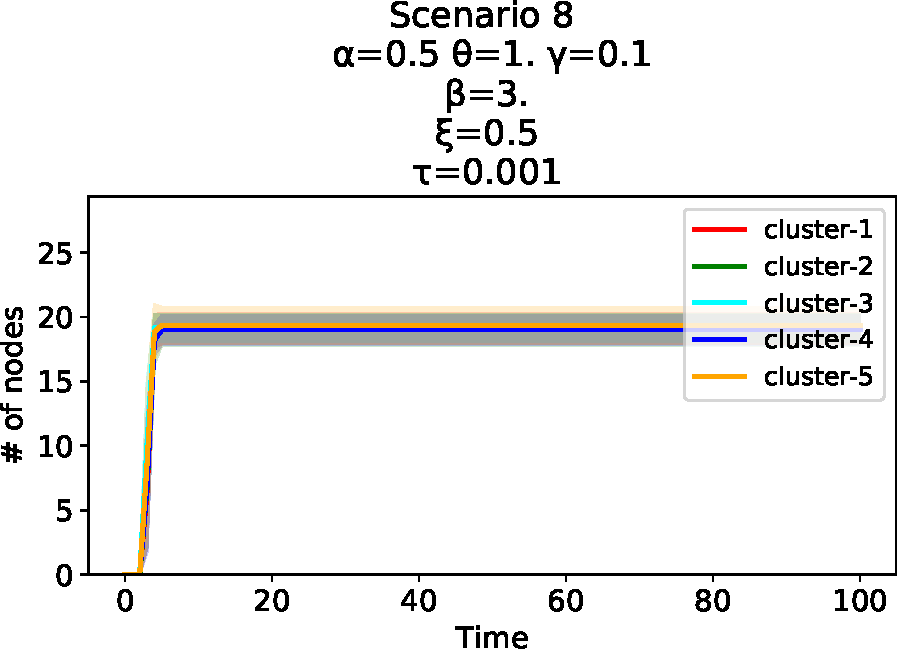
\includegraphics[width=\textwidth]{papers/swarm-intelligence2021/img/simulations/failScenario_0_034567_α-0.5_θ-1._γ-0.1_β-3._ω-0._ζ-0._ξ-0.5_τ-0.001}
  \end{subfigure}
  \hfill
  \begin{subfigure}[b]{0.32\textwidth}
    \centering
    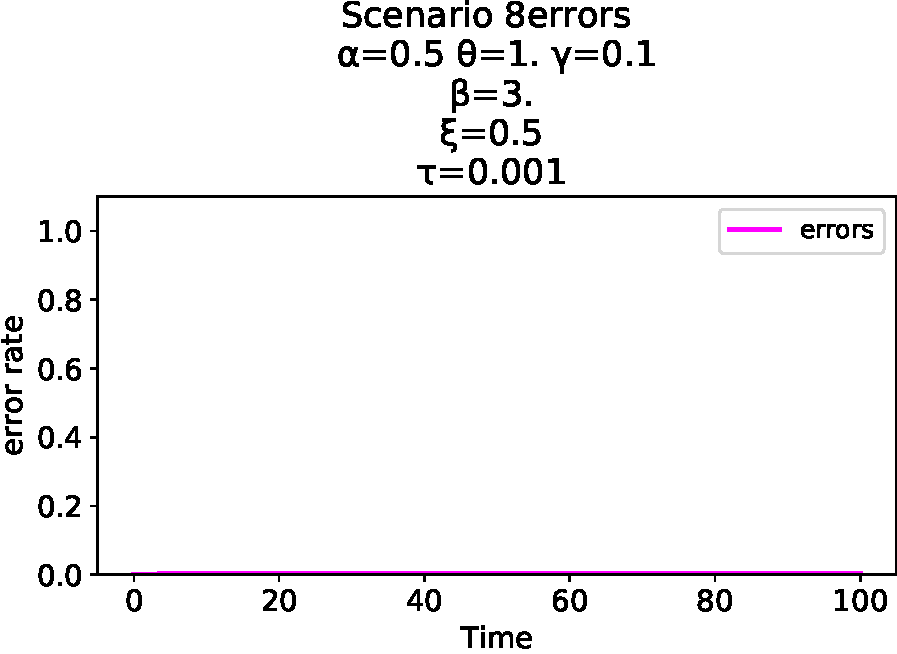
\includegraphics[width=\textwidth]{papers/swarm-intelligence2021/img/simulations/failScenario_0_08_α-0.5_θ-1._γ-0.1_β-3._ω-0._ζ-0._ξ-0.5_τ-0.001}
  \end{subfigure}
  \hfill
  \begin{subfigure}[b]{0.32\textwidth}
    \centering
    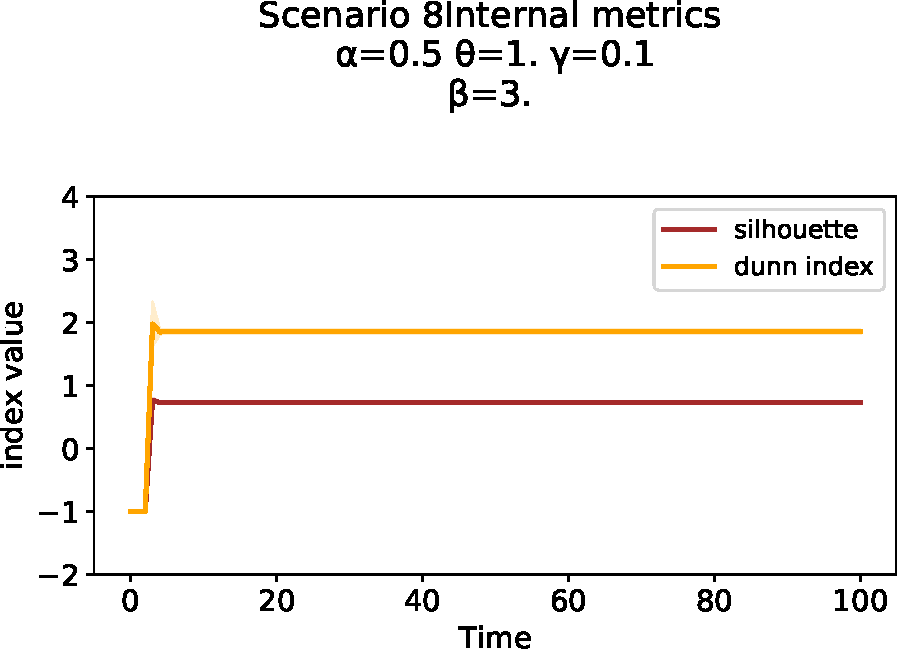
\includegraphics[width=\textwidth]{papers/swarm-intelligence2021/img/simulations/failScenario_0_0910_α-0.5_θ-1._γ-0.1_β-3._ω-0._ζ-0._ξ-0.5_τ-0.001}
  \end{subfigure}
  \caption{In-depth analysis of good simulation results. 
  In general, the algorithm produces good results. 
  \rev{In the case of movement and failures, the error can reach up to 10 per cent.}}
  
  \label{fig:good-simulation-results}
\end{figure}

\begin{figure}[!ht]
  %%% PROBLEM 1: thr %%% 
  \begin{subfigure}[b]{0.32\textwidth}
    \centering
    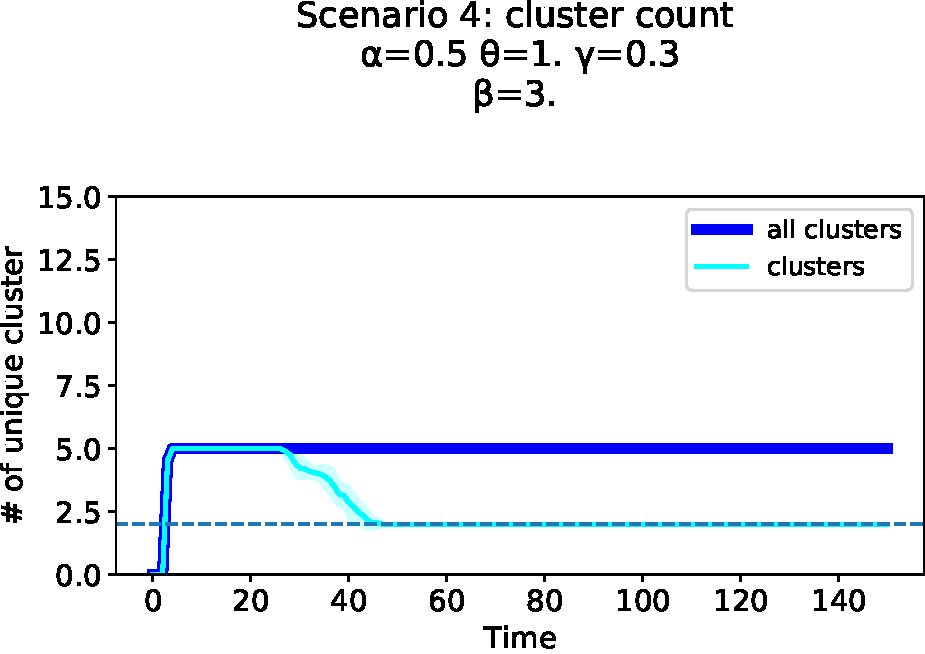
\includegraphics[width=\textwidth]{papers/swarm-intelligence2021/img/simulations/overlay_0_021_α-0.5_θ-1._γ-0.3_β-3._ω-0._ζ-0..pdf}
  \end{subfigure}
  \hfill
  \begin{subfigure}[b]{0.32\textwidth}
    \centering
    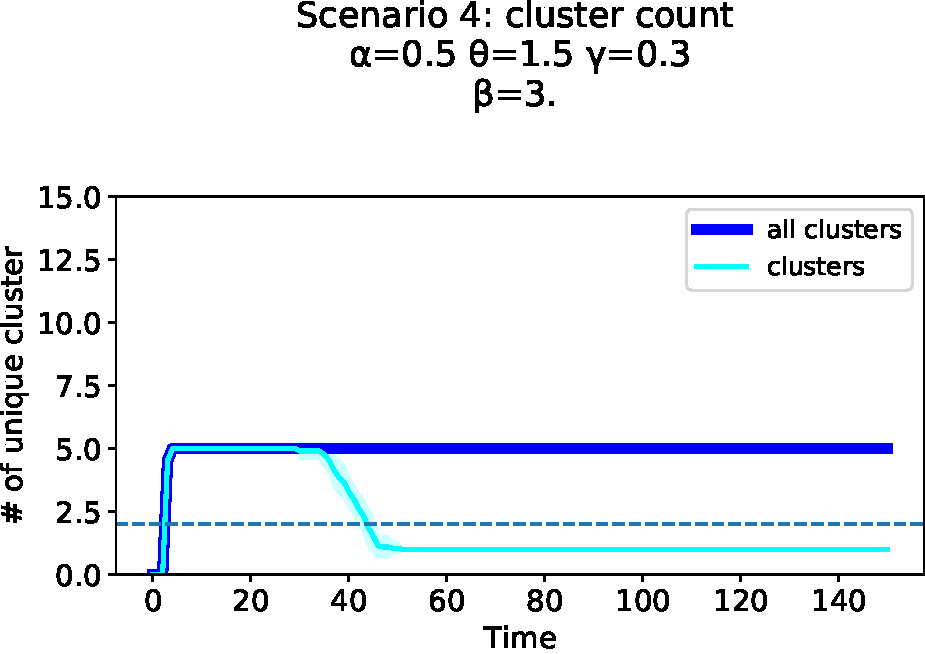
\includegraphics[width=\textwidth]{papers/swarm-intelligence2021/img/simulations/overlay_0_021_α-0.5_θ-1.5_γ-0.3_β-3._ω-0._ζ-0..pdf}
  \end{subfigure}
  \hfill
  \begin{subfigure}[b]{0.32\textwidth}
    \centering
    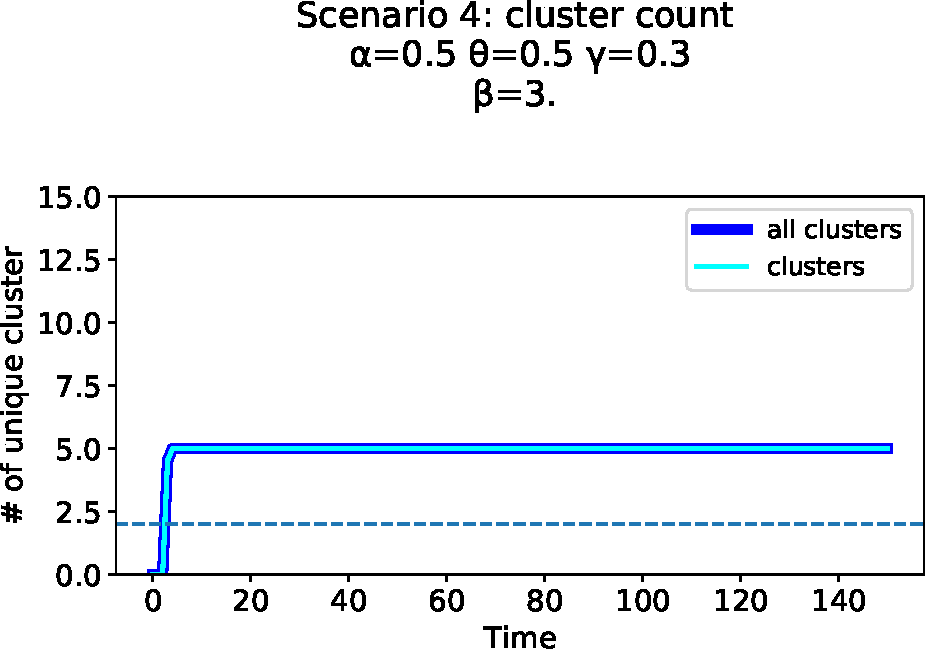
\includegraphics[width=\textwidth]{papers/swarm-intelligence2021/img/simulations/overlay_0_021_α-0.5_θ-0.5_γ-0.3_β-3._ω-0._ζ-0..pdf}
  \end{subfigure}
  %%% PROBLEM 2: density %%% 
  \begin{subfigure}[b]{0.32\textwidth}
    \centering
    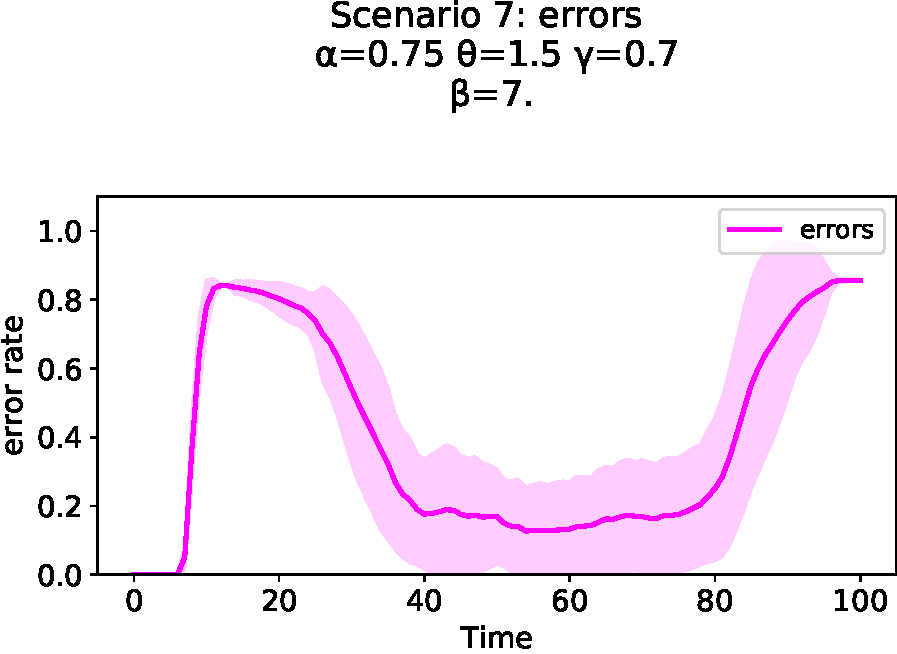
\includegraphics[width=\textwidth]{papers/swarm-intelligence2021/img/simulations/standard-updatable-errors_0_08_α-0.75_θ-0.5_γ-0.1_β-5._ω-0._ζ-0..pdf}
  \end{subfigure}
  \hfill
  \begin{subfigure}[b]{0.32\textwidth}
    \centering
    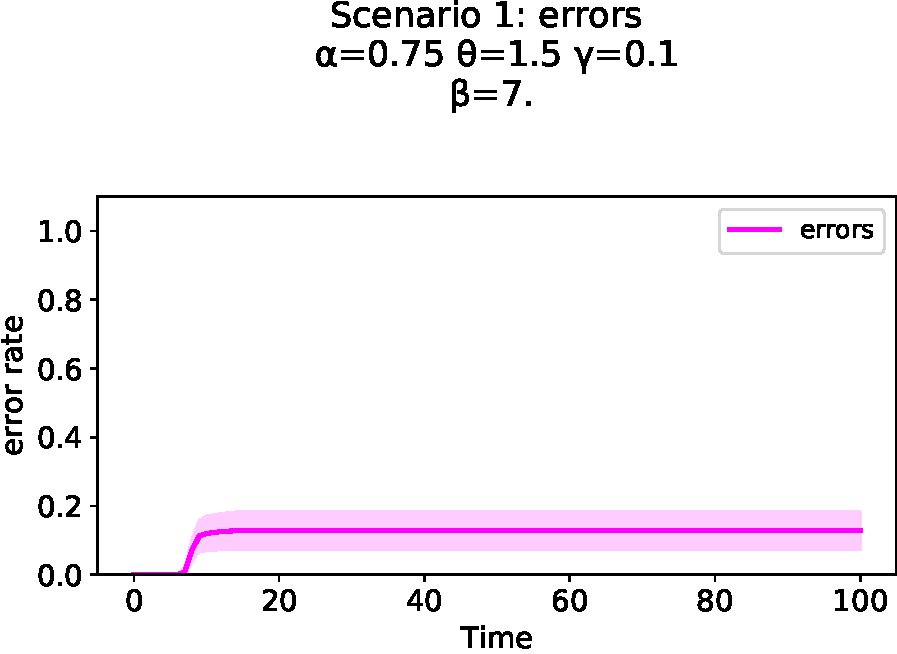
\includegraphics[width=\textwidth]{papers/swarm-intelligence2021/img/simulations/standard-errors_0_08_α-0.75_θ-1.5_γ-0.1_β-7._ω-0._ζ-0..pdf}
  \end{subfigure}
  \hfill
  \begin{subfigure}[b]{0.32\textwidth}
    \centering
    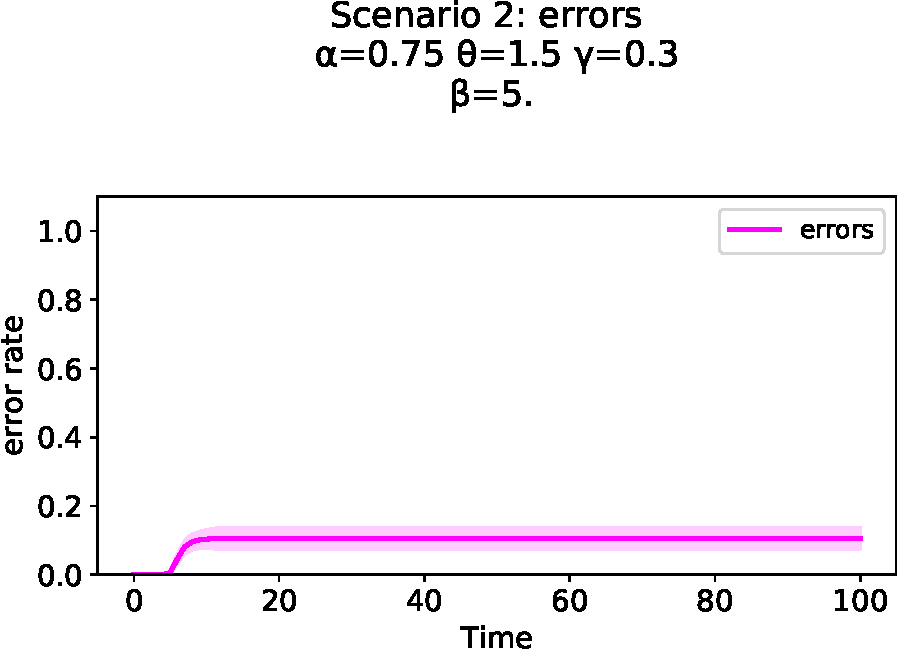
\includegraphics[width=\textwidth]{papers/swarm-intelligence2021/img/simulations/stretched-errors_0_08_α-0.75_θ-1.5_γ-0.3_β-5._ω-0._ζ-0..pdf}
  \end{subfigure}
  \\
  %% Focus 3: mobility
  \begin{subfigure}[b]{0.32\textwidth}
    \centering
    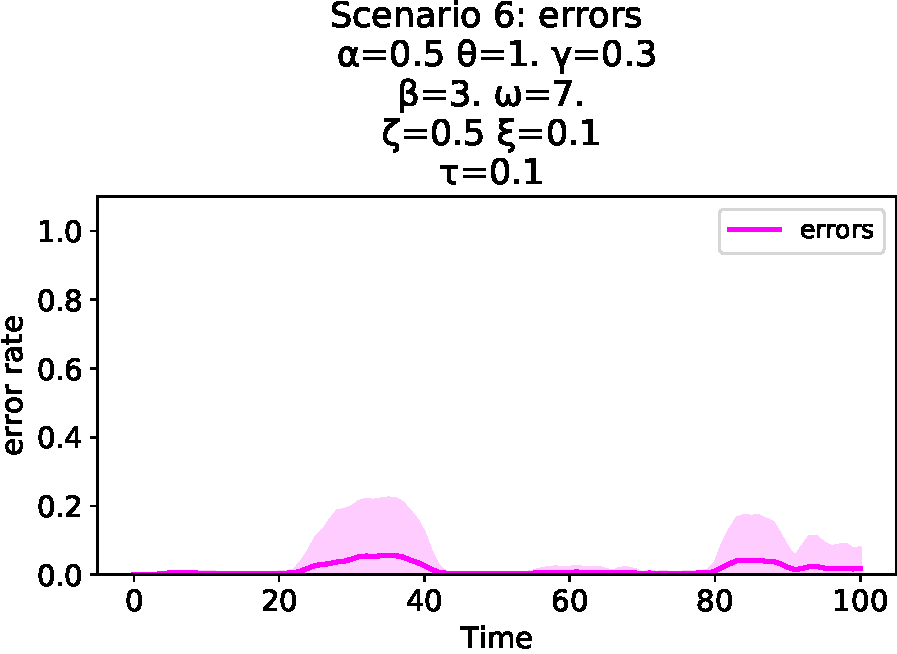
\includegraphics[width=\textwidth]{papers/swarm-intelligence2021/img/simulations/movement-errors_0_08_α-0.5_θ-1._γ-0.3_β-3._ω-7._ζ-0.5.pdf}
  \end{subfigure}
  \hfill
  \begin{subfigure}[b]{0.32\textwidth}
    \centering
    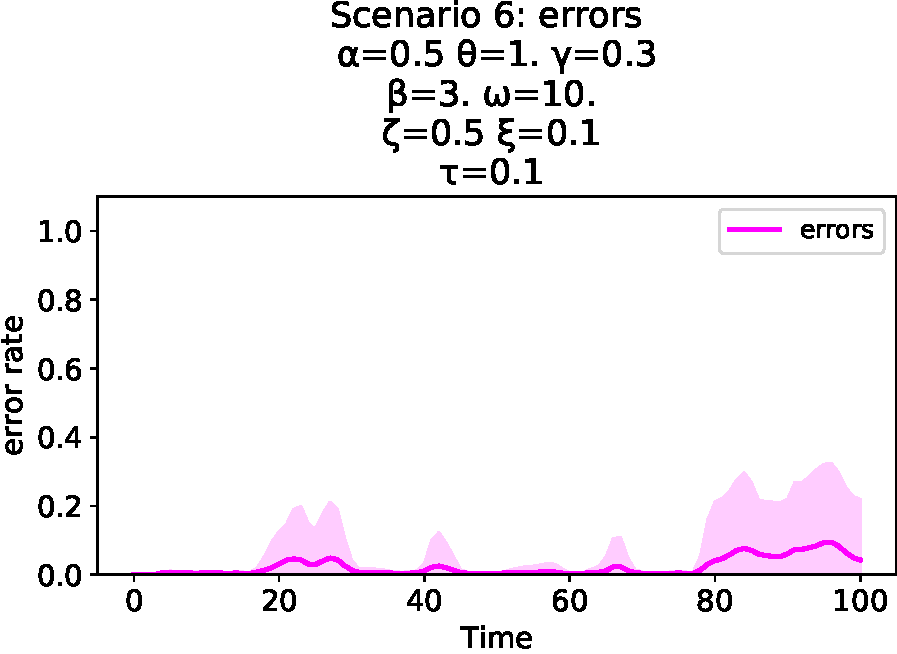
\includegraphics[width=\textwidth]{papers/swarm-intelligence2021/img/simulations/movement-errors_0_08_α-0.5_θ-1._γ-0.3_β-3._ω-10._ζ-0.5.pdf}
  \end{subfigure}
  \hfill
  \begin{subfigure}[b]{0.32\textwidth}
    \centering
    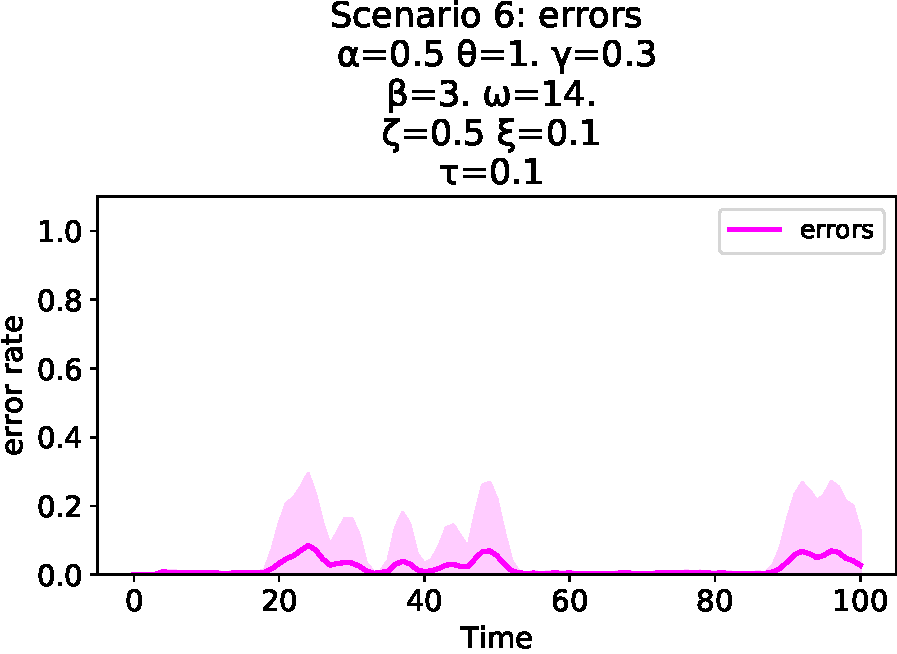
\includegraphics[width=\textwidth]{papers/swarm-intelligence2021/img/simulations/movement-errors_0_08_α-0.5_θ-1._γ-0.3_β-3._ω-14._ζ-0.5.pdf}
  \end{subfigure}
  \\
  %% Focus 4: movement range
  \begin{subfigure}[b]{0.32\textwidth}
    \centering
    \includegraphics[width=\textwidth]{papers/swarm-intelligence2021/img/simulations/movement-errors_0_08_α-0.5_θ-1.5_γ-0.1_β-3._ω-7._ζ-0.6.pdf}
  \end{subfigure}
  \hfill
  \begin{subfigure}[b]{0.32\textwidth}
    \centering
    \includegraphics[width=\textwidth]{papers/swarm-intelligence2021/img/simulations/movement-errors_0_08_α-0.5_θ-1._γ-0.1_β-3._ω-7._ζ-0.6.pdf}
  \end{subfigure}
  \hfill
  \begin{subfigure}[b]{0.32\textwidth}
    \centering
    \includegraphics[width=\textwidth]{papers/swarm-intelligence2021/img/simulations/movement-errors_0_08_α-0.5_θ-1._γ-0.7_β-3._ω-10._ζ-0.6.pdf}
  \end{subfigure}
  %% Focus 4: movement range
  \begin{subfigure}[b]{0.32\textwidth}
    \centering
    \includegraphics[width=\textwidth]{papers/swarm-intelligence2021/img/simulations/failScenario_0_08_α-0.75_θ-0.5_γ-0.1_β-7._ω-0._ζ-0._ξ-0.5_τ-0.001}
  \end{subfigure}
  \hfill
  \begin{subfigure}[b]{0.32\textwidth}
    \centering
    \includegraphics[width=\textwidth]{papers/swarm-intelligence2021/img/simulations/failScenario_0_08_α-0.75_θ-0.5_γ-0.1_β-7._ω-0._ζ-0._ξ-0.5_τ-0.1}
  \end{subfigure}
  \hfill
  \begin{subfigure}[b]{0.32\textwidth}
    \centering
    \includegraphics[width=\textwidth]{papers/swarm-intelligence2021/img/simulations/failScenario_0_08_α-0.75_θ-0.5_γ-0.1_β-7._ω-0._ζ-0._ξ-0.5_τ-0.5}
  \end{subfigure}
  \caption{Main examples of bad clustering results.
  In the first line, the images show different behaviour varying $\theta$.
  In the second line, the plots show how the algorithm does not handle well low-density robot swarms.
  In the third line, the charts show how the algorithm handles various movement speeds.
  The fourth line shows how the exploration range impacts the clustering results.
  \rev{Finally, the last line shows how failures impact performance.}
  }
  \label{fig:bad-simulation-results}
\end{figure}
The simulation results underscore the algorithm's capability to effectively partition the data into meaningful clusters. 
 As demonstrated in \Cref{fig:overview-results}, 
 our algorithm stabilizes to produce the correct number of clusters after a certain settling period. 
In the sections that follow, we concentrate on discussing the outcomes in relation to the evaluation goals outlined in \Cref{s:eval-goal}.
\paragraph*{Goal \ref{goal:1}: static sensing/spatial-based clustering}
Running the simulations of scenarios 1-5 we verified how much the clusters extracted follow the underlying temperature distribution in the static context.
 \Cref{fig:overview-results} shows that the algorithm correctly extracts the cluster number -- with the optimal parameters' configuration.
 Furthermore, observing \Cref{fig:good-simulation-results}, we can deduce that the cluster shape is correct too.
 Indeed, the Silhouette index tends to be 1 when the clusters are disjointed, and the error rate is negligible.

Here, $\theta$ plays a key role. Observing the behaviour of scenario 4 in \Cref{fig:bad-simulation-results},
 we see that with too low $\theta$ we overestimate the cluster numbers and,
 with a high level of $\theta$, we underestimate the cluster number.
 But this was the expected behaviour, as it depends directly on the trend of the target distributions.

Finally, Another important aspect is the density ($\alpha$) of the system.
 With a few nodes, candidate nodes may be positioned far from the cluster centre, thus identifying wider areas than expected.
\paragraph*{Goal \ref{goal:2}: robustness against node mobility \emph{and failures}}
When nodes have a low mobility and exploration range, the system is robust to node movements (\Cref{fig:good-simulation-results}).
 The exploring policy introduces errors, but the results are comparable to solutions where the nodes are stationary.
Moreover, even in case of failures, the clustering process is practically not affected at all.
However, in the worst case, mobility and failures lead to false positives (\Cref{fig:bad-simulation-results}).
 Indeed, some processes start in areas where the temperature is almost constant.
 Therefore, that process approximately covers the whole area (and hence produces a high error rate).
\rev{Scenario 8 is mainly influenced by the low-density situation.
 Indeed, in that case, removing nodes lead to not covering the whole system. }
\paragraph*{Goal \ref{goal:3}: robustness against temperature changes}
The result of scenario 7 is comparable to the static scenario.
 Indeed, \Cref{fig:good-simulation-results} shows that the cluster number is correct, and \Cref{fig:good-simulation-results} shows that the error rate is low, and the shape is accurate.
 The solution suffers from low-density values and wrong $\theta$ values as scenarios 1-5 (\Cref{fig:bad-simulation-results}).

\subsection{Discussion}
\label{sec:eval-discussion}

\rev{\subsubsection*{Simulations} \label{sec:eval-discussion-simulations}}
Ultimately, 
 our algorithm can support a certain degree of movement, \rev{sporadic failures},
 find various cluster shapes, 
 and cope with temperature changes in the optimal condition:
 high density ($\alpha$), limited exploration range ($\zeta$), and an appropriate value for in cluster threshold ($\theta$) value.

However, when drones move randomly, 
 the algorithm starts to produce sub-optimal cluster divisions since the nodes do not care about the cluster found,
 and they continue to explore the area.
%
But this could lead to becoming a false candidate and then starting an unwanted clustering process.
 Furthermore, it could be argued that uniform zones are part of a cluster that is not identified as there are no relative minima.
%
For this reason, when a node starts the process in a non-correct zone, the cluster identification will expand in the nearly whole system.
 This problem could be reduced by changing $\omega$ and $\zeta$ when the nodes belong to a cluster.

It is important to highlight that when \(\alpha\) is set to a low value, 
 the algorithm tends to produce poor cluster divisions, a phenomenon that becomes particularly evident in the presence of failures. 
 This limitation is inherent to our algorithm's design, 
 which relies on a centroid to initiate the clustering process.
% 
With a low \(\alpha\) value, 
 the likelihood increases that the node initiating the clustering process is distant from the true centroid of the cluster. 
 As a result, the expansion process may deviate from the underlying distribution, leading to a significant misclassification of nodes.

\subsubsection*{Hardware Deployment}
\label{sec:eval-discussion-deployment}
While we have not conducted experiments involving the clustering algorithm on a physical system, 
 insights can be gleaned from the physical deployment of FCPP~\cite{DBLP:conf/acsos/Audrito20}, a C++ library that provides an internal DSL for field-based programming. 
 This deployment was carried out in the context of an Industrial Internet of Things (IIoT) scenario~\cite{testa:pmcj:2022}. 
 The hardware used consisted of DWM1001C modules by Decawave, which are resource-constrained with a 64MHz ARM Cortex-M4 CPU, 512 KB of flash memory, and 64 KB of RAM. 
 Despite these limitations, the porting of FCPP was successful, and we were able to execute a field-based program with dynamic processes whose complexity is comparable to the clustering algorithm discussed in this paper~\cite{testa:pmcj:2022}.

The DWM1001C modules support BLE (Bluetooth Low Energy) and UWB (Ultra Wideband) for communication. 
 In the IIoT context, BLE was used for message exchange among neighboring nodes, while UWB was employed for distance estimation. 
 This distance data could be integrated into the current clustering algorithm using the \lstinline|gradient| function for multi-hop distance estimation.

Although the FCPP deployment experience has been promising, pointing toward the feasibility of deploying our clustering algorithm in a similar setting, 
 several differences between the two scenarios merit further investigation. 
 Firstly, the largest IIoT experiment involved only 20 nodes, 
 which may be insufficient to adequately assess the clustering algorithm
\section{Related Work}
\label{s:rw}
%
Coverage of related work is organized to separately cover\rev{:
 related swarm-based environment monitoring approaches (\Cref{s:rw:related-env-monitoring}),}
 related clustering models and problems (\Cref{s:rw:related-problems}),
 research work related to the sensing-based clustering problem we address (\Cref{s:rw:related-sensingbased-clustering}),
 research work related to field-based computing (\Cref{s:rw:related-approaches}),
 and related field-based algorithms (\Cref{s:rw:related-ac-algorithms}).

\rev{
\subsection{Swarm-based Environment Monitoring}
\label{s:rw:related-env-monitoring}
%
The approach proposed
 can be used
 to dynamically cluster a swarm,
 e.g.,
 to monitor an environment
 in a decentralized way.
%
Literature on swarm-based environment monitoring
 is ample~\cite{DBLP:journals/ram/DunbabinM12}.
%
In particular, various works leverage mobility and sparse sampling~\cite{DBLP:journals/ijrr/BestCPMF19,casadei2022coord-space-fluid,DBLP:conf/icra/KemnaRNYS17}.

In \cite{DBLP:conf/rss/GargA14},
 a persistent monitoring approach
 of environment phenomena
 with discontinuous dynamics
 is proposed.
%
It is
 based on optimally
 adapting a sparse set of
 sensing locations
 according to an evolving stochastic model of the environment.
%
In~\cite{DBLP:journals/ijrr/BestCPMF19},
 decentralized planning is used to support multi-agent active perception,
  which leverages movement to improve the quality of information gathering through effective choice of ``viewpoints'' in space and time.
%
In~\cite{DBLP:conf/icra/KemnaRNYS17},
 the authors focus on multi-agent coordination for informative adaptive sampling in unknown, communication-constrained environments (like lakes or oceans).
%
Their approach is based on dynamic, 
 decentralized Voronoi partitioning over a set of sampling locations, which are recalculated at synchronization points initiated through requests for surfacing events.
%
Though the approach of this paper could also be used to support \emph{sparse sampling}~\cite{casadei2022coord-space-fluid},
 it also aims at supporting the formation of spatially cohesive clusters for coordinated processing and/or action.
%
Moreover, 
 we do not aim at moving agents to appropriate sampling locations,
 but rather leave the agents to move autonomously (e.g., according to exploration policies)
 while having the collective clustering
 reflect the underlying phenomenon
 to support decision-making possibly beyond pure environmental sampling.
%
The use of Voronoi partitions in \cite{DBLP:conf/icra/KemnaRNYS17} differs from our clustering
 in that they leverage regions to limit
 the prospective sampling locations
 to be visited by each vehicle,
 while we actually want to define \emph{groups} of coordinating agents.
}

\subsection{Related Clustering Models and Problems}
\label{s:rw:related-problems}

Clustering is a well-known problem in data analysis and machine learning, 
 and has been widely studied in the literature~\cite{Jain:1999,DBLP:journals/sigkdd/Estivill-Castro02,Jain:2010}.
In a classical setting, the data to be clustered is stored in a single dataset, and a single algorithm (or agent) is in charge of finding the ``best'' clusters according to some optimization criteria.
 Each data point in the input data set is described by the values of a fixed set of {\em features}; 
 the number of such features constitutes the dimensionality of the data set and, typically, high dimensional data is harder to cluster meaningfully.

A characteristic of the clustering tasks considered in the present paper (and in general, of sensing-based methods, see the next section), 
 is that besides the sensed data,
 a main source of information is the spatial distance between the agents. 
 In~\cite{Thrun:2021}, the authors consider high-dimensional data sets that exhibit {\em natural clusters}, characterized by distances and/or density-based structures.
 They propose a semi-automated method whereby the clusters are automatically proposed and manually selected starting from a topographic visualization of the high-dimensional data.
 Notably, they use swarm intelligence for computing the topographic map, 
 while other techniques are adopted for the interactive process of clusters computation.

There are, however, several works that address swarm-based clustering, 
 using swarm intelligence for the clustering task itself~\cite{Martens:2011}.
 It is important to note that such methods (both those based on particle swarm optimization (PSO), and those based on ant colony systems (ACS)) exploit swarms just as a computational means for finding clusters in a data set.
 Their goal is not to cluster the elements of the swarm itself, 
  as it is the case for the present work, but to simulate a virtual swarm to find good quality clusters.

Some works directly address the clustering of swarms. 
 In~\cite{DBLP:journals/trob/HuBJAL21}, the clustering of a team of special agents (i.e., aerial drones) is part of a larger process that,
 after cluster formation, also involves formation tracking (i.e., tracking a target through a suitable formation), and containment control (i.e., surround ground agents cooperating in the mission).
 The method proposed to form clusters is based on a \emph{game-theoretic} framework named GRAPE. 
 A significant difference w.r.t. the present work is that the number (and nature) of clusters is determined by a given set of targets,
 while we do not assume such a priori knowledge.
Another significant work with similar goals is~\cite{DBLP:journals/tie/GeHZ18}, 
 where a team of agents must be partitioned into clusters organized as suitable {\em formations} (i.e., geometric spatial patterns).
 The proposed solution inter-mixes the determination of clusters and their formation (based, among other things, on the agents' dynamics), 
 assuming that the number and nature of such formations is known a priori.

Since we consider clustering over a given topology (network), 
 the problem can be related to graph-based clustering \cite{Zheng:2010}.
Graph-based clustering, however, assumes that the given graph can be partitioned into densely connected subgraphs that are sparsely connected to each other; i.e.,
it assumes that all the similarity information is expressed by the presence of edges between nodes (and, possibly, by their weights).
This is not necessarily the case with the networks formed by our swarms, 
 where connections are just determined by spatial distance, 
 and the clustering is strongly influenced by the sensed data.
Also, community detection methods can be viewed as clustering of the nodes of a graph representing a network of relations (e.g. a social network)~\cite{DBLP:journals/jnca/JavedYLQB18}.
Interestingly, unlike in generic graph-based clustering, communities can easily overlap, since a node (e.g., user) may belong to several communities at once.

\subsection{Related Work on Sensing-based Clustering}
\label{s:rw:related-sensingbased-clustering}

Sensing-based clustering typically applies to sensor networks that are distributed on a geographical area and exploit clustering mainly to reduce the communication bandwidth and/or energy consumption of the net.
 The role played by sensing a (possibly dynamic) geographic environment makes such problem and the proposed approaches to solve it relevant to the present work,
 although the agents considered here are themselves dynamic entities moving and acting across the space.

In \cite{DBLP:conf/ccnc/LinM07}, 
 the goal is to partition sensors for indoor monitoring and control. 
 The cluster heads are predetermined (based on the sources to be monitored and controlled),
 while cluster formation is periodically scheduled in order to adapt to changes in the sensed data.
%
In our work, instead, the cluster heads are not a priori given:
 they are determined according to the \emph{sensed data}
 (e.g., the agents perceiving local minima)
 and can change \emph{dynamically}
 (e.g., because a candidate withdraws and joins a different cluster).

The goal of \cite{DBLP:journals/tpds/GedikLY07} is, 
 instead, to obtain energy savings in data collection from a wireless sensor network by receiving values from only a subset of selected representatives and predicting the other valuer through automatically generated statistical models.
Cluster heads are chosen (probabilistically) based on the amount of energy they have. 
 Cluster formation is periodically scheduled, and the assignment of a sensor to a cluster is based on the distance from the head and the similarity of the sensed value with the head's value.
%
A work with similar goals is~\cite{DBLP:journals/ijdsn/CaiZ18}, 
 where again energy savings in a WSN is the primary motivation. 
 Here, the cluster heads are chosen based on residual energy level and data gradient.
 Moreover, an autoregressive prediction model for sensory data is maintained by each head to self-adjust temporal sampling intervals within the cluster.

A sensing-based clustering problem is also studied in~\cite{DBLP:journals/jaihc/KucukBSK20} where, 
 however, instead of being a high energy-constrained WSN, 
 the deployed system involves sensorized units and mobile phones able to upload all the relevant data to the cloud, through cellular and Wi-Fi connections. 
 In a disaster scenario, the mobile phones data is used to centrally compute density-based clusters that can inform the SAR (Search and Rescue) teams about the location of people in the area.

The {\em DyClee} approach described in~\cite{DBLP:journals/pr/RoaTG19} is also centralized. 
 The authors assume that streams of sensors observations (e.g. in an Industrial IoT) 
 are continually tracked by their system, 
 and are classified (e.g., as healthy or faulty) 
 based on a set of clusters that capture the patterns corresponding to different states. 
% 
The main focus is on the novelty detection problem, 
 or concept drift, which implies the ability to update the clusters as new behaviour is learned, while ignoring noise and occasional outliers. 
 The online clustering algorithm consists of two stages based, 
 respectively, on distance and density, and is {\em fully dynamic} in that it is able to create, eliminate, drift, merge, and split clusters as data is processed.

\subsection{Related Approaches and Programming Models}
\label{s:rw:related-approaches}

Programming swarms of agents is a difficult task, 
 because of the need of coordinating their local behaviours to achieve global, swarm-level goals.
%
In this work, we adopt the field-based computing and programming approach~\cite{DBLP:journals/jlap/ViroliBDACP19}
 for expressing self-organising, collective behaviour of swarms.
%
Our focus is on decentralized behaviour-based approaches (rather than automatic design methods like e.g. reinforcement learning),
 as surveyed e.g. in~\cite{DBLP:journals/swarm/BrambillaFBD13,DBLP:journals/jlap/ViroliBDACP19}
 and briefly in the following.

%
An approach to the problem that has proven to be quite effective is generative communication through tuple-based coordination models, 
 as offered, e.g., in the Linda language~\cite{linda} and its descendants; 
 essentially, several processes running on the same system can synchronize by writing and retrieving information in a shared (tuple-)space.
A derived idea is that of allowing programmability of the tuple space itself, so that the coordination logic of processes can be embedded in the communication medium--see, e.g.,~\cite{respect-scico2001}.
An obvious limitation of the mentioned approaches for the task of swarm programming is that they assume a central memory accessible by all the agents/processes. 
 However, the idea of tuple-spaces has been extended also to distributed systems, e.g., in the IBM TSpaces framework~\cite{Wyckoff:1998}.

An important feature of swarm systems is their adaptivity achieved through self-organization.
%
A support to build such kind of systems is offered by frameworks inspired by other sciences such as biology~\cite{tolksdorf2003using} and chemistry~\cite{DBLP:journals/alife/Sayama09}.
%
The field-based computing approach adopted in the present paper is based, instead, on the concept of {\em field}, borrowed from physics.
%
The related idea of a {\em field of tuples} has been implemented in the TOTA middleware~\cite{tota}.

As seen in this chapter, the field-based approach is particularly well suited to mobile, spatially situated agents.
%
A related (and precursor) thread of research of that of {\em spatial computing},
 where space is both an abstraction and a means for computation.
%
Spatial computing approaches have been largely surveyed in~\cite{SpatialIGI2013}.
%and particularly to the space-time computing model implemented in the Proto language~\cite{proto06a}, which can be seen as a direct ancestor of FC.
%
They are also related to \emph{macro-programming}~\cite{DBLP:conf/ipsn/NewtonMW07},
 where distributed systems as wholes are programmed by a centralized perspective.
%
For instance, a prominent related macro approach to swarm programming
 is Buzz~\cite{DBLP:journals/software/PinciroliB16},
 where swarms are first-class collection-like abstractions.

\subsection{Related Field-based Algorithms} %% TODO THESIS -- undestand if something might be introduced before this discussion or it could be ok to put everything here!! 
\label{s:rw:related-ac-algorithms}
Field-based computing has the peculiar ability to capture collective behaviours as functions operating on fields
and to compose them together as ``building blocks'' to address problems of increasing complexity~\cite{DBLP:journals/jlap/ViroliBDACP19}.
%
Of particular relevance for the present discussion is the implementation of the \emph{SCR (Self-Organising Coordination Regions)} pattern.
%
Most specifically, the SCR pattern can be denoted as a feedback chain S-G-C-G: leaders are elected (S); then, a gradient from leaders builds the communication structure (G); then, data from members (indirectly defined by the information path towards a leader) is collected towards leaders (C); then, data from leaders is propagated back to the members of the regions (G).
%
However, the SCR pattern is not limited to clustering (S-G part), but also regulates interactions within regions (C-G part).
%
Roughly, the sensing-based clustering algorithm
 covered in this work could replace the initial C-G composition
 that determines the system regions.

Similar to a clustering algorithm, 
 the S block~\cite{DBLP:conf/saso/MoBD18} provides a distributed mechanism to elect leaders from a set of candidates, 
 and to assign each remaining {\em user} node to a leader, 
 thus partitioning the system into regions. 
% 
The approach presented here is different in several respects: 
%
 first, the candidate leaders are determined by a characteristic of a \emph{sensed} measure (e.g., local minimum); 
%
 second, each candidate cluster head spawns an aggregate process to recruit other nodes within the cluster; 
% 
 finally, the other nodes can join more than one cluster, 
 based on the similarity of their sensed values with the ones sensed by leaders.

\section{Final Remarks}
\label{s:conc}

%\meta{ASSIGNED TO: Ferruccio / Mirko}

In this chapter, we precisely define and address
 the dynamic sensing-based mobile swarm clustering problem---an essential task in the context of \ac{cpsw}, to support the coordination of collective tasks based on environmental sensing data.
%
Most specifically,
 we use our language-based approach centred on aggregate computing to devise 
 a novel configurable meta-algorithm
 promoting self-organised clustering in a swarm
 of neighbouring-interacting agents.
%
The algorithm is evaluated on a set of synthetic environment configurations
 in the context of swarm robotics---a typical application domain for \ac{cpsw}.
%
In particular, we show that a swarm can autonomously
 create clusters reflecting the underlying dynamics of the  perceptible target phenomenon in the environment,
 and can deal with changes in the swarm topology and environment.
%
The subsequent chapter will introduce a general programming pattern for distributed sensing and actuation in Cyber-Physical Social Wearable (\ac{cpsw}) systems. 
 This pattern aims to provide a comprehensive solution for addressing the challenges associated with \ac{cpsw} programming.

%\printbibliography